\documentclass[12pt,a4paper]{report}
\usepackage[utf8]{inputenc}
\usepackage{subcaption}
\usepackage{caption}
\usepackage{float}
\usepackage{amsmath}
\usepackage{amsfonts}
\usepackage{amssymb}
\usepackage{graphicx}
\usepackage{bookmark}


%\usepackage[left=2.500cm, right=2.5cm, top=3.00cm,bottom=3.00cm]{geometry}

%\usepackage[export]{adjustbox}
%\usepackage{wrapfig}

\hypersetup{
	colorlinks=false,
	pdfborder={0 0 0},
}
\graphicspath{ {./pic/} }
\usepackage{array}
\newcommand{\dd}[1]{\mathrm{d}#1}
 
\title{From Chinese Painting to Bas-relief }
\author{Yunfei Fu}
\date{ }

\begin{document}
 

\begin{titlepage}
	
	\newcommand{\HRule}{\rule{\linewidth}{0.5mm}} % Defines a new command for the horizontal lines, change thickness here
	
	\center % Center everything on the page
	
	%----------------------------------------------------------------------------------------
	%	HEADING SECTIONS
	%----------------------------------------------------------------------------------------
	
	\textsc{\LARGE BOURNEMOUTH UNIVERSITY}\\[1.5cm] % Name of your university/college
	\textsc{\Large TRANSFER DOCUMENT}\\[0.5cm] % Major heading such as course name
 
	
	%----------------------------------------------------------------------------------------
	%	TITLE SECTION
	%----------------------------------------------------------------------------------------
	
	\HRule \\[0.4cm]
	{ \huge \bfseries From Chinese Painting to Bas-relief}\\[0.4cm] % Title of your document
	\HRule \\[1.5cm]
	
	%----------------------------------------------------------------------------------------
	%	AUTHOR SECTION
	%----------------------------------------------------------------------------------------
	
	\begin{minipage}{0.4\textwidth}
		\begin{flushleft} \large
			\emph{Author:}\\
			Yunfei \textsc{Fu} % Your name
		\end{flushleft}
	\end{minipage}
	~
	\begin{minipage}{0.4\textwidth}
		\begin{flushright} \large
			\emph{First Supervisor:} \\
			Dr. Hongchuan \textsc{Yu}\\
			\emph{Second Supervisor:}\\
			 Pro. Jian Jun \textsc{Zhang}
		\end{flushright}
	\end{minipage}\\[4cm]
	
	% If you don't want a supervisor, uncomment the two lines below and remove the section above
	%\Large \emph{Author:}\\
	%John \textsc{Smith}\\[3cm] % Your name
	
	%----------------------------------------------------------------------------------------
	%	DATE SECTION
	%----------------------------------------------------------------------------------------
	
	{\large \today}\\[3cm] % Date, change the \today to a set date if you want to be precise
	
	%----------------------------------------------------------------------------------------
	%	LOGO SECTION
	%----------------------------------------------------------------------------------------
	
	%\includegraphics{Logo}\\[1cm] % Include a department/university logo - this will require the graphicx package
	
	%----------------------------------------------------------------------------------------
	
	\vfill % Fill the rest of the page with whitespace
	
\end{titlepage} 
%\newpage  \section*{\centering ABSTRACT}

Bas-relief is an art form part way between sculpture and painting, in this research , we present a new approach for generating aesthetically pleasing bas-reliefs from brush paintings. We do not aim to recover exact depth values for objects in the paintings, which is a hard computer vision problem, requiring assumptions that are rarely satisfied. Instead, our approach exploits the concept of brush strokes, making strokes possible to generate 3D bas relief proxies separately suitable for recomposing in art design. Different paintings have different stroke patterns. Understanding the rules will improve the success rate of a wider range of paintings.Currently, our research focus on brush paintings with relatively sparse and clear strokes. 

As showed in Figure \ref{pip}, the approach performs in three steps: First,  based on the point cloud of the input image in RGB space, we select the palette colors of the input brush painting, and based on the palette colors we decompose a input image into different layers with transparency,  Second,  the original painting is decomposed into element brush strokes by applying modified MSERs segmentation.Based on our observation, alpha map is more suitable for our MSERs segmentation, so the segmentation is based on the transparency. Third, based on the segmented brush strokes,  Shape from Shading algorithm has been applied to generate the depth map of each stroke.  finally, based on those 3D strokes , we can edit the generated bas relief. For editing,we have already generated the 3D proxies for each MSER region, namely, the extracted 2D brush region, so, we can change the depth of specific stroke on bas relief,we can also stitch them on each other based on the user input and change the shape of a certain stroke with given indicated skeleton. By doing so, we fulfill the request of recomposition in bas-relief design.The resulting 3D proxies of brush strokes are sufficient to evoke the impression of the consistent 3D shapes,so that they may be further edited in 3D space. 
Experiments show that our method can effectively generate digital bas-reliefs for a range of input images, including some Chinese paintings and rose-mailing paintings.
We also demonstrate the utility of the resulting decompositions for image recoloring and image object insertion and animation.

\begin{figure}[H]
\centering
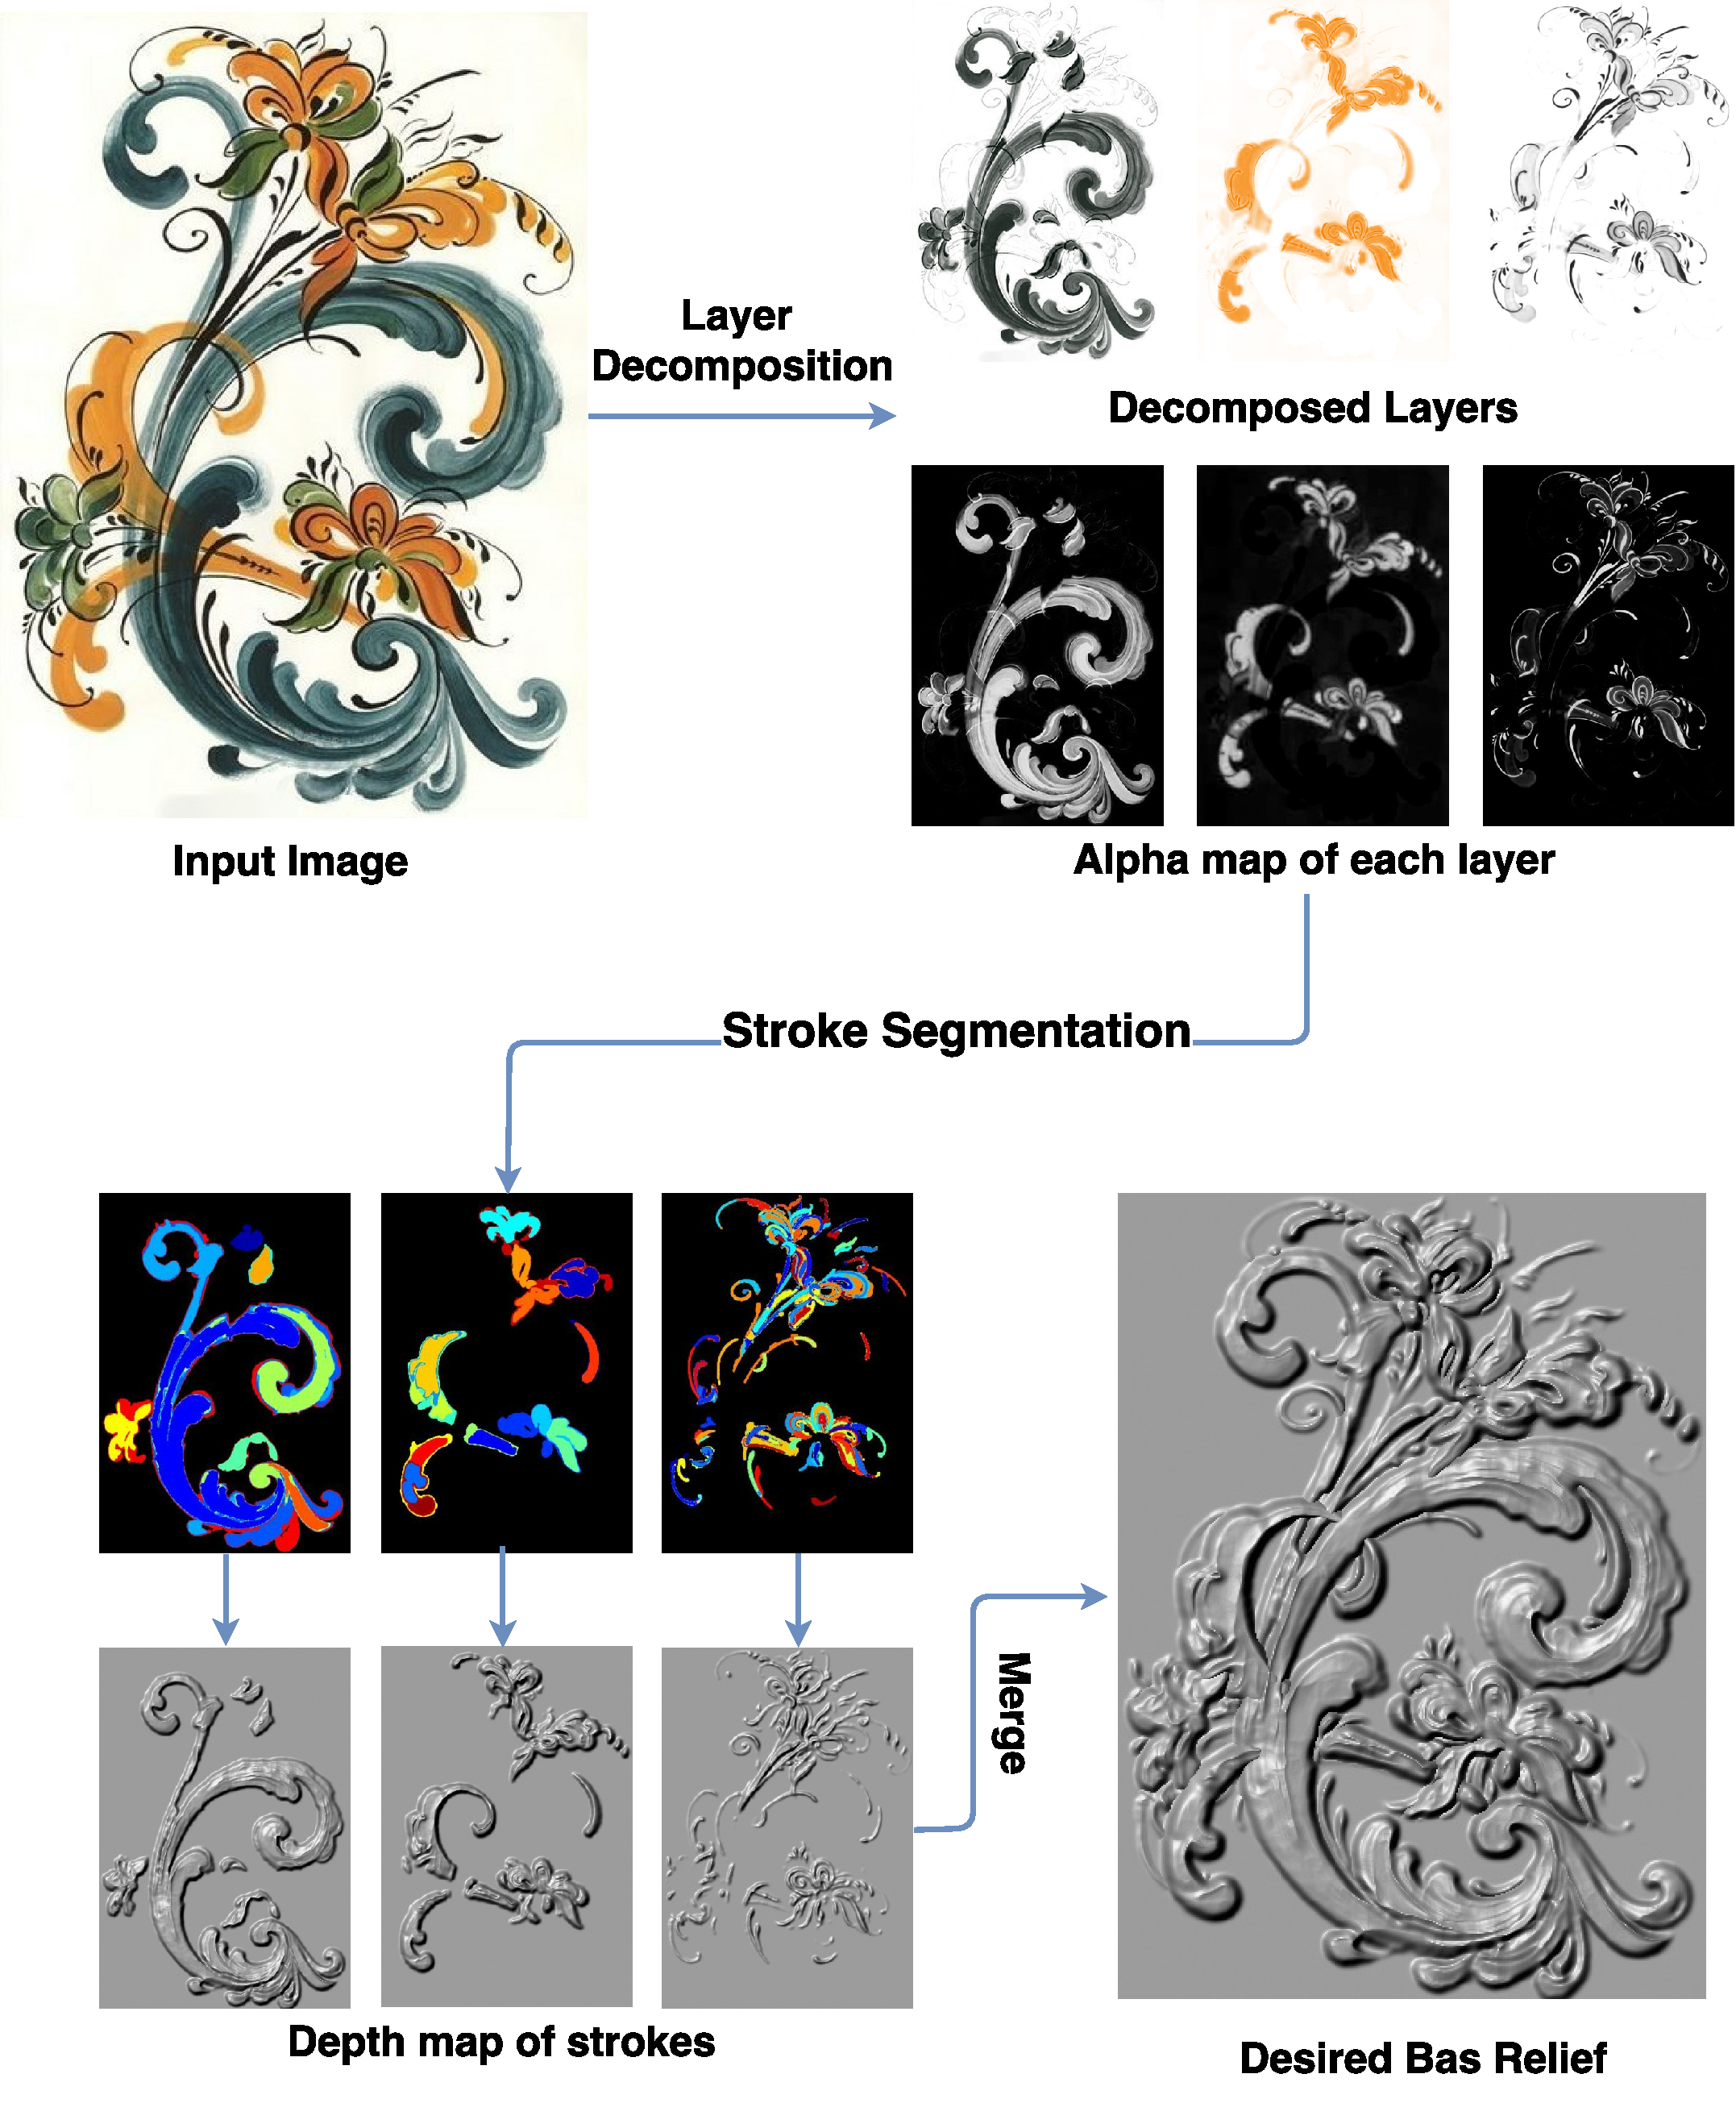
\includegraphics[scale=0.4]{overview.pdf}
\caption{Pipeline Overview}
\label{pip}
\end{figure} 
 
\newpage


 

 
\newpage  \section*{\centering ABSTRACT}
Bas-relief is an art form part way between 3D sculpture and 2D painting. We present a new approach for generating a bas-relief from a single Chinese brush painting.We do not aim to recover exact depth of a painting, which is a tricky computer vision problem, requiring assumptions that are rarely satisfied.Instead, our approach exploits the concept of brush strokes, making each brush stroke possible to generate a correspond bas-relief proxies(depth map of brush strokes),and combine the depth map of brush strokes together to construct the bas-relief model. To segment brush strokes in 2D paintings, we apply layer decomposition and stroke segmentation by imposing boundary constraints, which can make strokes smooth and complete. The resulting brush strokes are sufficient to evoke the impression of the consistent 3D shapes on bas-relief, so that they may be further edited in 3D space. Currently, our research focus on Chinese brush paintings.We demonstrate our approach on a variety of Chinese brush paintings, and even some other suitable styles include rosemaling paintings and certain watercolor paintings, our approach is able to produce convincing bas-reliefs.\\
As a secondary application, we show how our brush stroke extraction algorithm could be used for image editing.And our brush stroke extraction algorithm is specifically geared to handling paintings with highly characteristic brushstrokes, in addition to Chinese paintings, other suitable styles include rosemailing paintings and certain van Gogh's oil paintings.

\begin{figure}[H]
\centering
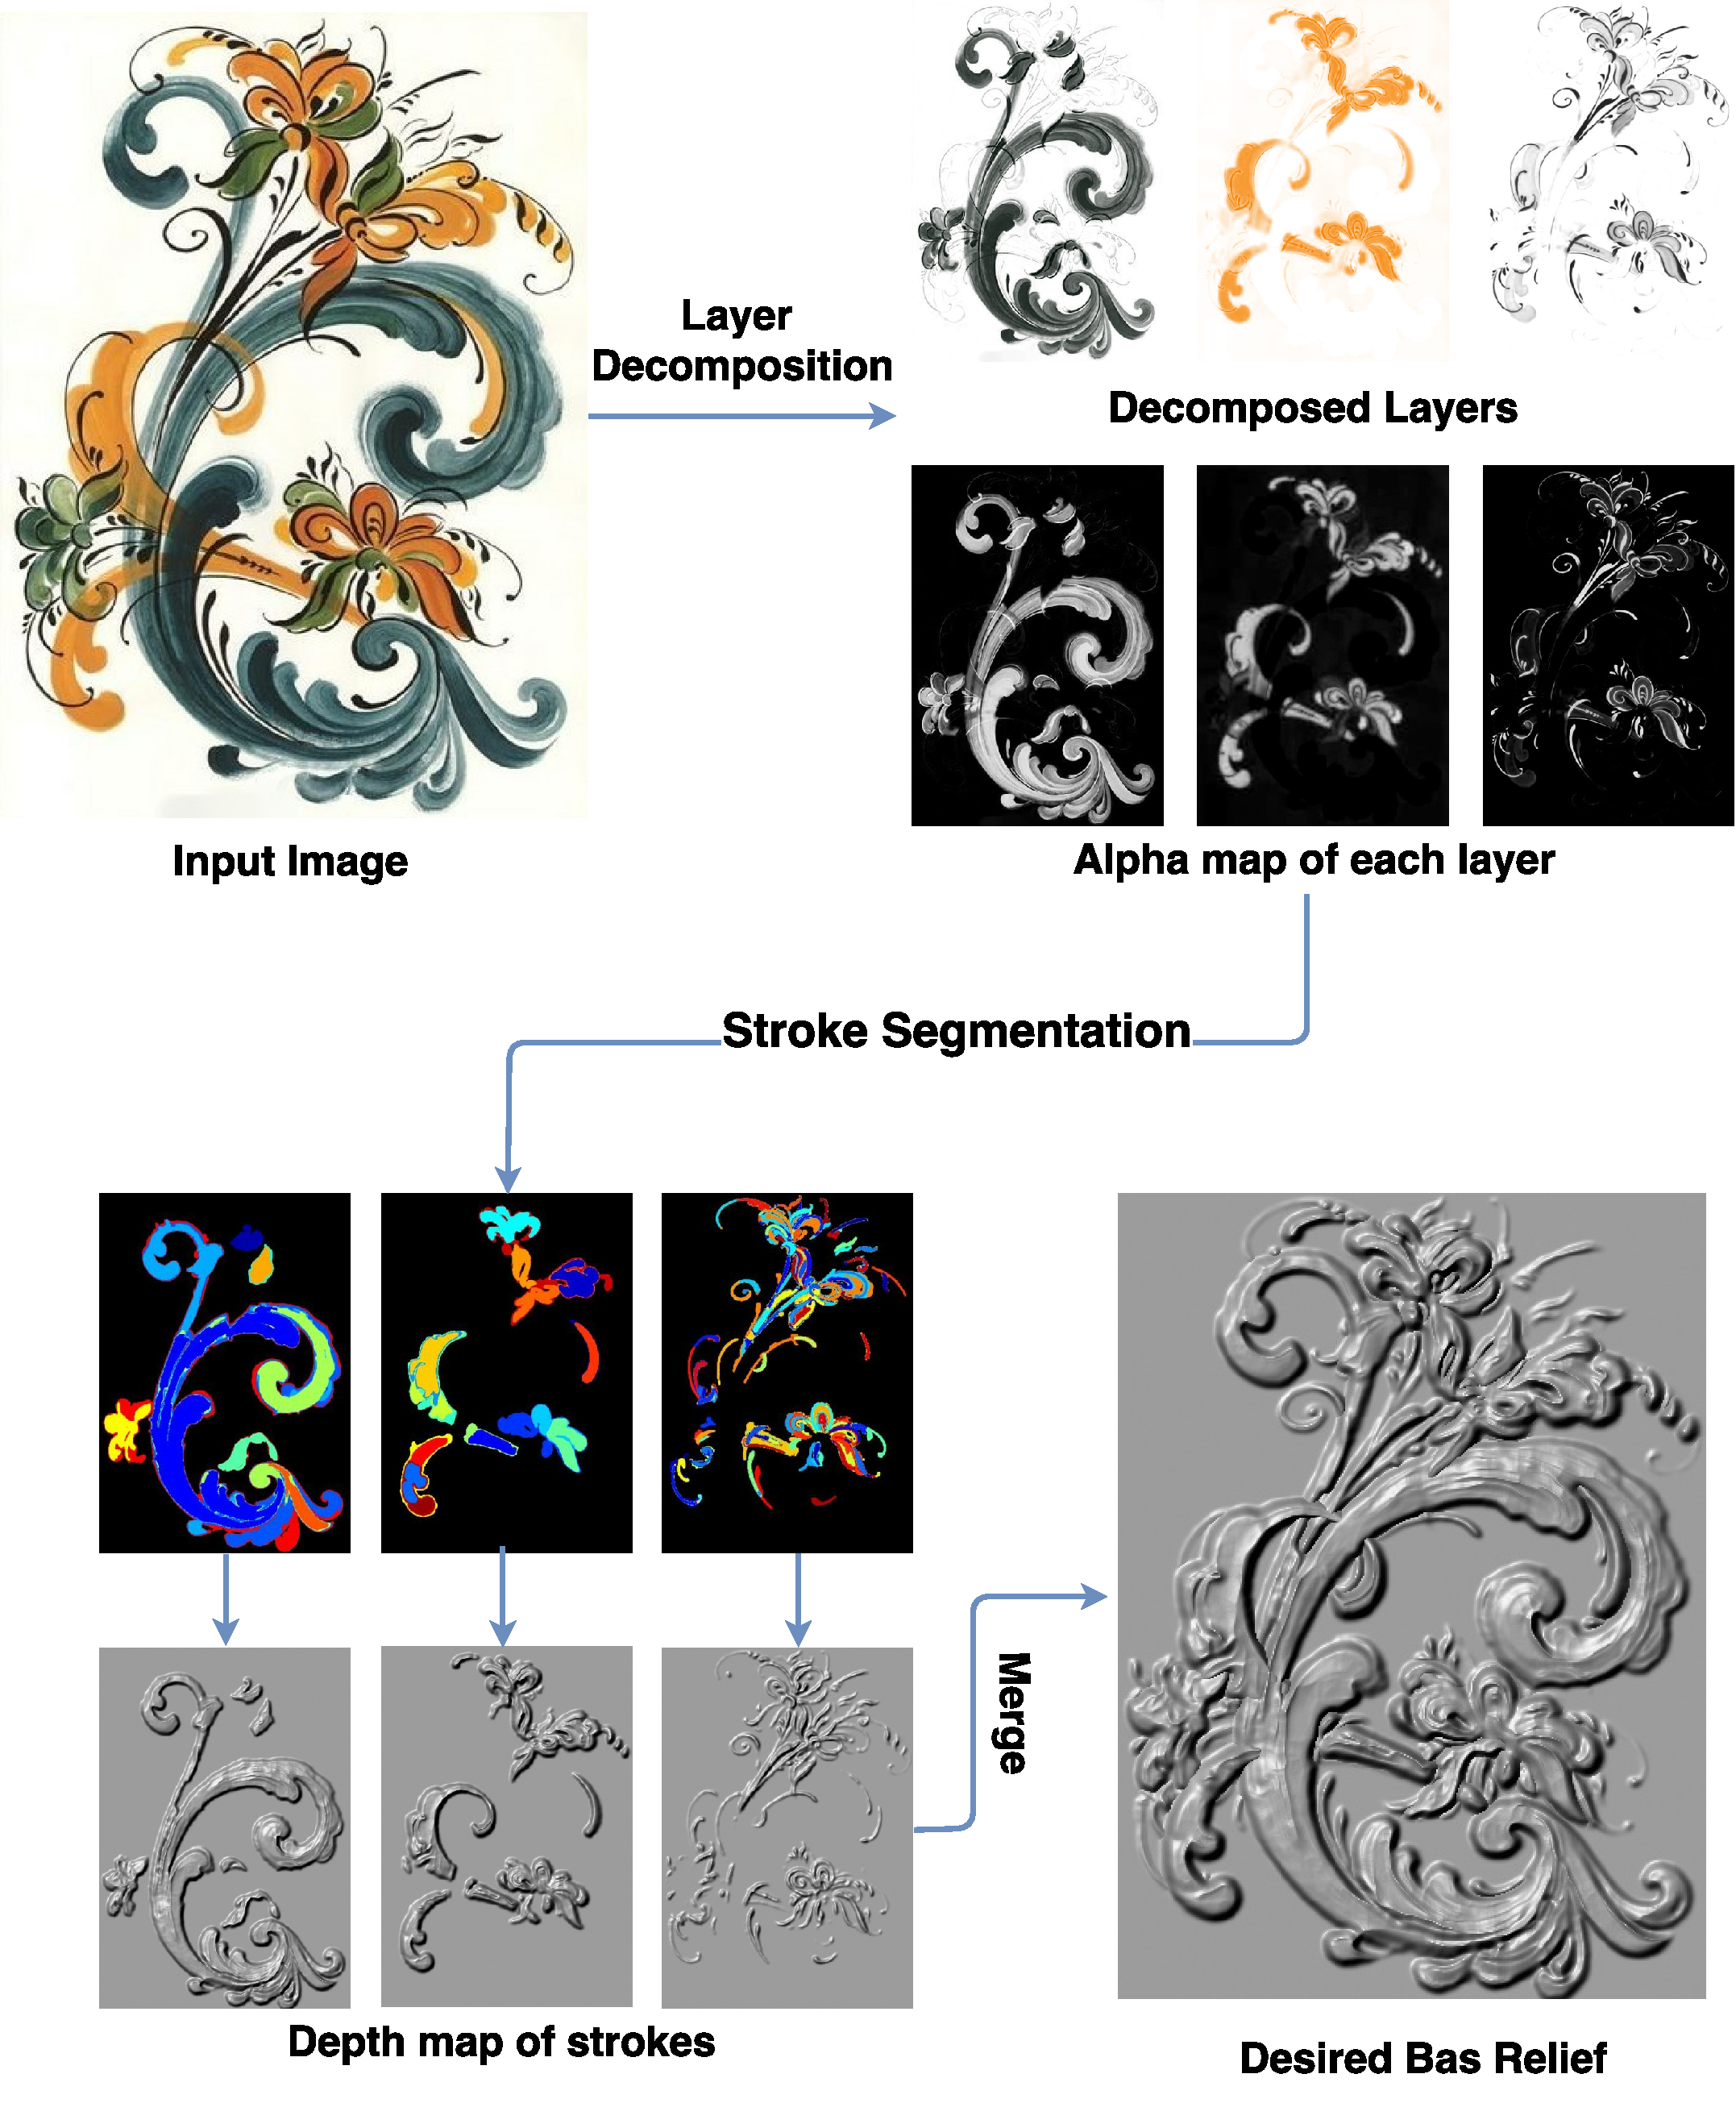
\includegraphics[scale=0.4]{overview.pdf}
\caption{Pipeline Overview}
\label{pip}
\end{figure} 
 
\newpage


 

 
\newpage  \input{./sec/terminology.tex}   
\newpage  \tableofcontents
\newpage  \listoffigures
%\newpage  \listoftables

\newpage  \chapter{INTRODUCTION}

\section{Background}
Relief is a method of sculpture in which forms are carved into a
relatively flat surface. In essence, it creates a bridge between a full 3D sculpture and a 2D painting. On this spectrum,high relief is closest to full 3D, whereas flatter artworks are described as bas-relief. Among all the sculpture forms, bas-relief is the closest to 2D paintings\cite{kerber2009feature} \cite{barron2012color}.\\ \\
Bas-relief sculpting has been practiced for thousands of years.Since antiquity, artisans from many ancient cultures(including Greek, Persian, Egyptian, Mayan, and Indian art) have created bas-reliefs.
Today bas-reliefs are commonly found in a variety of media, commemorative medals, coins, souvenirs, 2.5D animation,and artistic sculptures for blind people. However, crafting bas-reliefs is a laborious, challenging and time-consuming process. And with the commonly and cheaply available 3D printing facilities, there is a growing trend in the need of bas-relief art products.There are many ways to reach the same goals more easily with the help of computers. In the past two decades, a sizable amount of research has gone into developing bas-relief generation methods\cite{benzaid2017analysis}.\\ \\ 
Bas-relief is regarded as an art form part way between 3D sculpture and 2D painting \cite{benzaid2017analysis}\cite{barron2012color}\cite{weyrich2007digital}\cite{kerber2009feature}\cite{kerber2012computer}. Correspondingly, the existing bas-relief generation methods can also be classified in two different categories with respect to their input\cite{benzaid2017analysis}:
\begin{itemize}
 \item 3D model based : using a 3D model (sculpture) as input 
 \item 2D image based : using a 2D image as input 
\end{itemize} 
\subsection{3D model based:} \textbf{How to generate a bas-relief from a 3D sculpture? }The 3D model based bas-relief generation methods focus on such a problem,in which a 3D sculpture is considered as a 3D digital model.   The generation of bas-relief from 3D model was first studied in the pioneering work of \cite{cignoni1997computer}, then various existing 3D model based methods have demonstrated how to compress 3D model into bas-relief \cite{weyrich2007digital}\cite{kerber2009feature}\cite{song2007automatic}\cite{sun2009bas} . However,this approach requires a 3D model as a starting point.
\subsection{2D image based:}\label{2dimagebased} On the other hand,\textbf{ how to generate a bas-relief from a 2D painting?} \\ There have been some bas-relief generation approaches available based on a 2D image \cite{zeng2014region}\cite{wu2013making}  \cite{alexa2010reliefs}\cite{wu2008interactive}.  These approaches almost follow the “bas-relief ambiguity”\cite{belhumeur1999bas}, that is, roughly speaking, from a frontal view the sculpture looks like a full 3D object while a side-view reveals the disproportional depth. 
A 2D painting can be considered as a image,however,these image based methods are focusing on general photograph from real scene,assuming illumination and reflectance are known, and the input image is formed from lighting and shading, which obviously unsuited for 2D paintings.And the generated bas-relief is a single depth map or mesh, which makes it hard for user to edit. \\
Some research focus on bas-relief generation from a line drawing \cite{kolomenkin2011reconstruction}\cite{varley2002estimating}\cite{malik1987interpreting}\cite{sykora2014ink}. However,line drawing based methods generate bas-relief without consideration for surface details: their approaches are limited to using information contained in a line drawing, which is not suited for paintings containing information such as color,texture and stroke shape. \\ \\
Reconstructing a surface given a single 2D image is an ill-posed problem in general. As described in most of the papers on 2D image based algorithms, the problem that manifests itself immediately is that there is no complete knowledge of the depth within a single image.However, with the purpose of generating bas-relief with acceptable quality, there are several factors to be considered specifically for the framing of the problem.\cite{benzaid2017analysis} describes the some core important factors in the bas-relief generation process: depth information, silhouettes and edges,fine details.\\
\textbf{Depth information:} Within a single image there is no complete knowledge of the depth. A reasonable interpretation must be determined in some manner. \\ 
\textbf{Silhouettes and Edges:} Generally, silhouettes and edges are used for separate object and background and generating a reasonable contrast between the foreground objects and the background as a starting establishment for interpreting heights. \\
\textbf{Fine Details:} Many images will contain many small features and details within the subject of the image. In the process of generate bas-relief from 2D images,small features and details are preferable to maintain.Examples are features like texture of a hand or the shininess of an apple. \\ 
In our work, we evaluate our result and compare with other alternative methods based on these three factors, see Section \ref{compare}. \\ \\ 

\section{Aim and Challenges}
As mentioned above, bas-relief is considered as a art form part way between 2D painting and a full 3D sculpture\cite{benzaid2017analysis}\cite{weyrich2007digital}\cite{kerber2009feature}\cite{kerber2012computer}\cite{zeng2014region} .And among all the sculpture forms, bas-relief is the closest to 2D paintings,as claimed by \cite{kerber2009feature} \cite{barron2012color}, while how to generate bas-relief from  paintings remains a problem .\\ 
The aim of our research is to provide a method to generate a bas-relief from a Chinese painting automatically. We also argue that because most Chinese paintings are produced with individual brush strokes, generating bas-relief surface from each brush stroke would preserve the original features of the painting.\\ 
A Chinese painting can be regarded as the union of brush strokes \cite{xu2006animating}. Most Chinese paintings are typically sparse with each brush stroke drawn very purposefully\cite{smith1997art},and each stroke exists on its own as a piece of art\cite{girshick2004simulating}.
Differing from the other bas-relief generation methods, our method will preserve this very feature by generating bas-relief surfaces from the brush strokes individually. 
This however demands to conquer several challenges.\\ 
First, unlike photograph,opacity of brush strokes is a important feature of Chinese painting. It is desired to preserve this feature on bas-relief.\\ Second,unlike previous 2D image based methods focusing on photograph, a Chinese painting does not obey the rules of lighting and shading, which increase the difficulty to mimic the details on bas-relief surface. \\Third, each brush stroke covers a region on the canvas and they may overlap each other, some quite heavily in a painting. To make sure the information is retained, every brush stroke has to be faithfully extracted. \\  \\

\section{Motivation}
The motivation of this research comes from three sides.\\First,as mentioned above, bas-relief is regarded as a art form part way between 2D painting and a full 3D sculpture, as claimed by many previous works \cite{benzaid2017analysis}\cite{weyrich2007digital}\cite{kerber2009feature}\cite{kerber2012computer}\cite{zeng2014region}. Research so far has been primarily done based on a 3D model,and some other methods based on a single photograph\cite{zeng2014region}\cite{wu2013making}  \cite{alexa2010reliefs}\cite{wu2008interactive} or a line drawing \cite{kolomenkin2011reconstruction}\cite{varley2002estimating}\cite{malik1987interpreting}\cite{sykora2014ink} as input. However,how to generate bas-relief from artistic paintings remains a problem .\\
Second, due to the various styles of painting, it is difficult to come up with a general bas-relief generation method suitable for all 2D paintings. Some paintings may be too abstract for bas-relief generation. One the other hand, for traditional Western painting style developed in the Renaissance,which emphasizes realism\cite{chu2004real}, previous 2D image based methods may easily handle.\\
On the other hand,the style and philosophies of Chinese paintings have influenced other painting styles \cite{chu2004real}. Study bas-relief generation from Chinese painting will naturally push forward the research frontier of bas-relief generation from other painting. \\
Third, Bas-relief generation has wide applications in making objects such as commemorative medals, coins, souvenirs, and artistic sculptures for blind people.With the commonly and cheaply available 3D printing facilities, there is a growing trend in the need of bas-relief art products. On the other hand, and as input of our bas-relief generation method, the digital image of Chinese paintings are easily accessible on the Internet.    \\
Therefore, designing an efficient method for bas-relief generation from Chinese painting is important both theoretically and practically.\\ \\

As mentioned above, previous bas-relief generation methods have demonstrate how to generated bas-relief from 3D models,photographs and line drawings. In contrast, this research is the first attempt to automatic generate bas-relief from a Chinese painting. \\
In contrast with previous 2D image based methods, our algorithm is also the first attempt to generate bas-relief from opacity, and we demonstrate that in Chinese painting, opacity can preserve more details than intensity. \\
Accompanying with this method, we have proposed an algorithm for brush stroke extraction.The major difference between our brush stroke extraction with the previous works is that our algorithm is based on a reformulated layer decomposition algorithm, which makes it capable of extraction overlapped brush strokes without the prior knowledge of brush strokes. And we demonstrate the our method have a better performance in brush stroke extraction comparing with another notable work  \cite{li2012restoration} (see Section  \ref{comparevan}).  \\
Most Chinese paintings are typically sparse with each brush stroke drawn very purposefully\cite{xu2006animating}, and such a feature can be found other painting styles,such as rosemailing painting\cite{smith1997art}. So our method is also suitable for rosemailing painting, as shown in Section \ref{more results} and Section \ref{editing}. 

\section{Document Structure}
The organization of the document is as follows:\\
Chapter 1: Introduction. This section provides the background, the motivation, aim and challenges made in current research.\\
Chapter 2: Literature Review. This section classifies and reviews related previous works in a systematic way.\\
Chapter 3: Overview of proposed approach. This section explains the methodology selected and defines some basic concepts used in the research.\\
Chapter 4: Layer Decomposition. This section introduces concept "Layer Decomposition" in this research, which is the basis of the proposed algorithm.\\
Chapter 5: Extraction of Brush strokes. This section describes the proposed algorithm of brush stroke extraction.\\
Chapter 6: Depth map and '3D strokes'.  This section shows how to generate the individual depth maps of extracted strokes. \\
Chapter 7: Results. This section reviews the up-to-date results based on proposed the method.\\
Chapter 8: Conclusions and Future work. This section concludes the progress up-to-date and discusses possible future work.
\newpage 
%\newpage  \chapter{INTRODUCTION}

Relief sculpting has been practiced for thousands of years.Since antiquity, artisans from many ancient cultures(including Greek, Persian, Egyptian, Mayan, and Indian art) have created bas-reliefs (Figure \ref{bas:his}).Today bas-reliefs are commonly found in a variety of media in architecture, industrial design and coins. However, the production of bas-reliefs is currently a costly and time-consuming process, requiring skilled sculptors and engravers.Even with the advent of computer-driven techniques providing a foundation for automation in bas-relief, making the design of bas-relief sculptures remains largely in the hands of artists.

As an artistic form, relief spans the continuum between a 2D  painting and a full 3D sculpture\cite{weyrich2007digital}. On this spectrum, alto-relievo (high relief) is closest to full 3D, whereas flatter artworks are described as basso-relievo (low relief, and also called bas-relief), as showed in Figure \ref{bas:his}. Among all the sculpture forms, bas-relief is arguably the closest to 2D paintings, as claimed by\cite{kerber2009feature} and\cite{barron2012color}.
 
\begin{figure}[H]
	\centering
	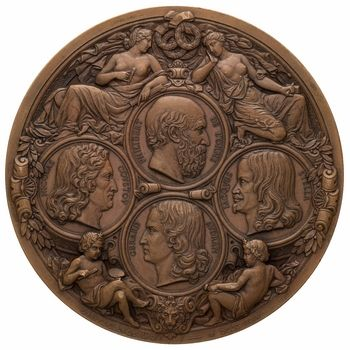
\includegraphics[height=0.2\textheight]{bas.jpg}
	~~~~
	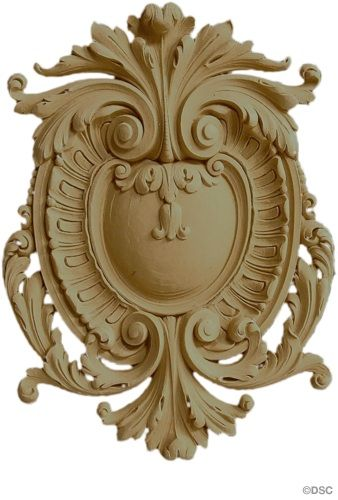
\includegraphics[height=0.2\textheight]{bas2.jpg}
	\caption{Bas-relief}
	\label{bas:his}  
\end{figure} 

Currently, most existing bas-relief production methods focus on compressing 3D scenes/models into surfaces with a small depth\cite{weyrich2007digital}and\cite{kerber2009feature}. This approach requires a 3D model as a starting point. 

Another option is to generate bas-reliefs directly from 2D images.There have been some image based bas-relief production approaches avail	able in\cite{zeng2014region}\cite{wu2013making} and \cite{alexa2010reliefs}. These approaches almost follow the “bas-relief ambiguity”\cite{belhumeur1999bas}, that is, roughly speaking, from a frontal view the sculpture looks like a full 3D object while a side-view reveals the disproportional depth. 

While most image based method are focusing on general photograph, which unsuited for specific problems for brush paintings, such as spatial occlusion (i.e. one stroke occludes other strokes in the paining to demonstrate the depth perception) and stroke transparency. A another clear shortcoming is current image based methods can’t take the artistic intent into account, as all what they do is to inferring the height information from the image. Concerning reproduction or modifying of an artistic painting, it is crucial that the style of the originals is preserved, which is not considered in existing image-based methods. However, little is done in the area of bas-relief generation from artistic paintings, as maintaining the styles of the brush paintings proves much trickier than simply manipulating the height of the contour lines. In the case of bas-reliefs, although there is no 3D model available, pseudo 3D effect reflecting the style and subtlety is crucial in preserving the artistic essence.

The aim of our research is to provide the bas-relief sculptors with a new tool allowing them to convert and recompose existing brush paintings to bas-reliefs. We also argue that because traditional paintings are produced with individual strokes, ‘3D bas-relief strokes’ will enable them to ‘paint/sculpt’ a bas-relief naturally, especially if they wanted to quickly convert an existing painting into a relief. With the commonly and cheaply available 3D printing facilities, there is a growing trend in the need of bas-relief art products.
A brush painting can be regarded as the union of a set of hypothetical strokes by a brush \cite{xu2006animating}. Differing from the other bas-relief generation methods, our method will honor this very feature by constructing the brush strokes individually as 3D geometric entities. This however demands to conquer several challenges. First, each brush stroke covers a region on the canvas and they may overlap each other, some quite heavily in a painting. To make sure the information is retained, every stroke has to be faithfully extracted. Second, spatial occlusion has to be dealt with, since artists are used to depicting it through controlling the transparency of strokes as one of the art elements. Third, as an artistic tool, the generated bas-relief should be further editable allowing the artist to rearrange, tweaking and reshaping the extracted strokes.

The shape, color and opacity of a stroke vary due to the shape and firmness of the brush as well as the forces the artist imposes. Although these variables add the complexity to stroke extraction, stylized strokes often follow distinct patterns. For example, Rosemaling paintings, a typical example of brush painting popular in North Europe, is a traditional form of decorative folk art that originated in the rural valleys of Norway. The Rosemailing designs use C and S strokes, feature scroll, flowing lines, floral designs, and both subtle and vibrant colors. The brush strokes may further be viewed as graphical objects which are meaningful with respect to the objects the painting portraits. Moreover, each stroke is clearly visible due to both subtle and vibrant colors. The similar properties may be found in some Chinese brush paints.
To extract the strokes from a brush painting, we need to identify and segment the overlapped strokes. We will then generate the depth map for every stroke separately using the shape from shading (SFS) technique on the opacity. All the strokes are finally merged together to yield the resulting bas-relief with the original 2D painting preserved. Our contributions include,
\newline
(1) Extraction of brush strokes. We develop a novel method to extract brush strokes from input paintings with palette analysis and decomposed layers.
\newline
(2) 3D modeling of brush strokes. We develop a novel method which may entirely construct every stroke in 3D based on the opacity of paintings.
\newline
(3) Recomposition in bas-relief design. Artists may redefine the brush strokes’ order and shapes by sketches, which enable recomposition in bas-relief design, making it a useful tool for sculpture artists.



\section{Thesis Structure}

The organization of the document is as follows:

Chapter 1: Introduction. This section provides the background, the motivation and the contribution made in current research.

Chapter 2: Literature Review. This section classifies and reviews related previous works  in a systematic way.

Chapter 3: Overview of proposed approach. This section explains the methodology selected and defines some basic concepts used in the research.

Chapter 4: Layer Decomposition. This section introduces concept "Layer Decomposition" in this research, which is the basis of the proposed algorithm.

Chapter 5: Extraction of Brush strokes. This section describes the proposed algorithm of brush stroke extraction.

Chapter 6: Depth map and '3D strokes'.  This section shows how to generate the individual depth maps of extracted strokes. 

Chapter 7: Results. This section reviews the up-to-date results based on proposed the method.

Chapter 8: Conclusions . This section concludes the progress up-to-date.

Chapter 9: Future work. This section discusses possible future work about high relief and 3D painting.
 
\newpage  \chapter{LITERATURE REVIEW}
This chapter reviews notable bas-relief generation methods classified into two categories, methods based on 3D model and method based on 2D image, which are reviewed in section \ref{ref3D} and section \ref{ref2dimage} respectively. The structure of these bas-relief generation methods is shown in Figure \ref{liter-review-stru}. Following with section \ref{sectionbss} which reviews notable brush stroke extraction methods and some relative works.
\begin{figure}[H]
	\centering
	\includegraphics[width=15cm]{liter-review.jpg}
	\caption{Bas-relief generation from brush strokes}
	\label{liter-review-stru}
\end{figure}

\section{Bas-relief Generation from 3D Model}\label{ref3D}
A significant amount of methods has been considered bas-relief generation from 3D model,\cite{cignoni1997computer} firstly proposed a method which  creates bas-relief models by linearly compressing (squeezing) the
depth map of 3D models. This method fails to handle the depth gap between in 3D models and the output bas-reliefs can not successfully preserve the  details on 3D models. 
Some researchers considered bas-relief generation as a geometry counterpart of the  high dynamic range (HDR) image compression problem widely studied in computer graphics\cite{song2007automatic}. This approach calculates the differential coordinates of the input 3D models, then HDR image process method is applied to compress the 3D models. The output bas-relief can preserve salient feature and de-emphasize the others,but sometimes the bas-relief can be distorted and exaggerated. 
The methods proposed in \cite{kerber2009feature}\cite{kerber2012computer} work on the gradient domain of depth map of 3D models, and rely on the combination of a saliency measure and a feature enhancement technique. These methods produce generally satisfactory bas-relief output,and preserve the features of 3D models, although again some areas can be over-emphasized. 
\cite{sun2009bas} generate the bas-relief with a optimized contrast-limited adaptive histogram equalization (CLAHE) method,in which the depth map of 3D model is compressed . Local contrast of depth map can be enhanced in this method,however, the detail preservation requires high resolution depth map from 3D model. \\ \\ 
These 3D model based methods can often generate bas-relief with acceptable quality , but they all require inputs in the form of 3D models, which are often difficult and time-consuming to prepare, and obviously unsuited for bas-relief generation from 2D paintings. 

\section{Bas-relief Generation from 2D Image}\label{ref2dimage}
Automatic bas-relief generation from 2D image has recently become a significant research topic. Researches have explored recovering depth information from images specifically for the purpose of generating bas-reliefs.\newline
\subsection{Photograph Based Methods}
Some methods generation bas-relief from a photograph \cite{zeng2014region}\cite{wu2013making} \cite{alexa2010reliefs}\cite{wu2008interactive}. And the very importance part of these methods is generating bas-relief surface based on shape from shading(SFS) algorithm. SFS is a relative classic way for 3D shape recovery; see Zhang's survey \cite{zhang1999shape}.  The computation process normally involved with several concepts : depth $Z(x,y)$, surface normal $n_x,n_y,n_z$ ,and surface gradient $p,q$. The depth can either be considered as distance from viewpoint to query surface or the height from surface to default $x-y$ plane. The normal is perpendicular to the surface gradient, namely $\left( n_x,n_y,n_z\right) * \left( p, q ,1\right)^T =0  $ , the surface gradient is the changing rate of depth in $x$ and $y$ direction.

Shape from shading (SFS) is able to recover the shape of an object from a given single image, assuming illumination and reflectance are known (or assuming reflectance is uniform across the entire image). Many methods have been developed, which may be categorized into four PDEs models\cite{prados2003perspective}, (1) orthographic SFS with a far light source \cite{lions1993shape}; (2) perspective SFS with a far light source\cite{prados2004unifying}; (3) perspective SFS with a point light source at the optical center\cite{prados2003perspective}; (4) a generic Hamiltonian. However, SFS is an ill-posed problem. The notable difficulty in SFS is the bas-relief ambiguity\cite{belhumeur1999bas}, that is, the absolute orientation and scaling of a surface are ambiguous given only shading information. To amend it, many SFS algorithms impose priors on shape, depth cues produced by a stereo system, or assume that the light source, the surface reflectance, and the camera are known\cite{zhang1999shape} \cite{alldrin2007resolving} \cite{johnson2011shape} \cite{barron2012color}.\\ \\
Unfortunately,these photograph based methods assume  illumination and reflectance are known, and the image is formed from lighting and shading, which may work well for realistic photographs rather than paintings,especially for Chinese painting. Simply applying SFS method is not enough to generate bas-relief with acceptable quality .  

\subsection{Line Drawing Based Methods}
Line drawing is a drawing made exclusively in solid lines. Rather than generating bas-relief from a photograph from real scene,some researches focus on bas-relief generation methods from line drawing.
Kolomenkin et al.\cite{kolomenkin2011reconstruction}  aims to reconstruct a model from a complex line drawing that consists of many inter-related lines. At first, they extract the curves from line drawing. Then, junctions between lines are detected and margins are generated. By analyzing the connectivity between boundaries and curves, they reduce the problem to a constrained topological ordering of a graph. From these boundaries and curves with given depth, they use smooth interpolation across regions generate the bas-relief surface. Similarly, line labeling methods has been applied for shape construction from line drawings  \cite{varley2002estimating}\cite{malik1987interpreting}\cite{sykora2014ink}. A labeling process would classify segmented lines into different labels, such as concave, convex and occluding, and these labels can give clues for the shape generation of bas-relief. 
\cite{sykora2014ink} proposed a bas-relief generation method consists of six main steps: segmentation, completion, layering, inflation, stitching, and grafting.This method combines user indications and shape inflation to model smooth bas-relief shapes from line drawings. \\ \\ 
However,line drawing based methods do not consider how to generate bas-reliefs with surface details: their approaches are limited to using information contained in a line drawing, which are not suited for brush strokes which contain information such as color,texture and stroke shape. 

\subsection{Gradient and Intensity Based Methods}
Wang et al.\cite{wang2010image} demonstrate a method by constructing bas-reliefs from 2D images based on gradient operations. In their research image gradients were calculated, then by smoothing gradients to smooth shape changes. Finally , they boost fine features with user input masks.
The height image was constructed modified height map. The pixel heights are compressed, and a triangle mesh representing the bas-relief is determined by placing a vertex at each pixel position. Most features can be preserve by proposed method, but no consideration is made for the front-to-back or overlapping relationship between different image regions. \newline
\cite{li2012restoration} present a two-level approach for height map estimation from the rubbing images of restoring brick and stone relief.  The relief is separated into low and high frequency components. The base relief of the low frequency component is estimated automatically with a partial differential equation (PDE)-based mesh deformation scheme. The high frequency detail is estimated directly from rubbing images automatically or optionally with minimal interactive processing. This method works well for reliefs based on stone rubbing images, but is unsuited to general photographs or paintings.

\section{Brush Stroke Extraction}\label{sectionbss}

To the best of our knowledge, there is lack of study on extracting brush strokes from paintings. We give a brief overview of the work related to the relevant topics, i.e. decomposing images into layers and stroke extraction, which are employed in our implementation. In digital image editing, layers organize images. However, scanned paintings and photographs have no such layers. Without layers, simple edits may become very challenging.\\
Richardt et al.\cite{richardt2014vectorising} present an approach to produce editable vector graphics, in which the selected region is decomposed into a linear or radial gradient and the residual, background pixels . \cite{mccann2009local},\cite{mccann2012soft}present two generalized layer decomposition methods, which allow pixels to have independent layer orders and layers to partially overlap each other.\cite{tan2016decomposing} present a layer decomposition method based on RGB-space geometry. They assume that all possible image colors are convex combinations of the paint colors. Computing the convex hull of image colors and per-pixel layer opacities is converted into a convex optimization problem. Thus, method in \cite{tan2016decomposing} can work well without prior knowledge of paint colors. However the proposed method simply focus on layer decomposition not stroke extraction, how to extract the brush stroke remains a problem.\\ 
Li et al.\cite{li2012rhythmic} describe a method based on seed growing for brush stroke segmentation.Starting from seed coordinates, neighboring pixels are visited by exploiting a region-growing-based approach with a variable threshold, which is initialized at a predefined and automatic updated by a shape validation method. In this research,they generated manually marked brush strokes using 10 example regions from van Gogh's paintings, and they define two parameters in order to evaluate the accuracy of extracted brush stroke. In section \ref{comparevan}, we compared our method with this method.  \\
Xu et al.\cite{xu2006animating} aims at decomposing Chinese paintings into a collection of layered brush strokes, with an assumption that at most two strokes are overlapping. However, their approach requires a good amount of prior knowledge of shape and order of strokes.And it requires professional artists to build a brush stroke library which makes it a challenging and time consuming process. While our method needs no brush stroke library, and our segmentation is based on multiple layers which more than two brush strokes could overlap each others(Figure \ref{mser:alpha}). \\ \\
Most Stable Extremal Regions (MSERs) algorithm\cite{matas2004robust} has been proved to be a very efficient way in stroke segmentation from scene text images\cite{neumann2011text}\cite{gomez2013multi}, 
and the revised version has been widely used in stroke segmentation of handwritten characters\cite{gomez2016fast}.\\
The Most Stable Extremal Regions (MSERs) algorithm\cite{matas2004robust} was used for establishing correspondence in wide-baseline stereo.\cite{donoser2006efficient} introduced the data structure of the component tree in it and further developed it as an efficient segmentation approach, which prunes the component tree and selects only the regions with a stable shape within a range of level sets.\\
However, it is likely that MSERs may fail in segmentation with the following scenarios,\newline (1) two adjacent regions with the similar intensity; \newline (2) the region with a high transparency. \newline
(3) Moreover, like the other existing segmentation approaches, the MSERs algorithm encounters over-segmentation issue as well. \\
To tackle these challenges, the coherent lines method \cite{kang2007coherent} is introduced into MSERs in our algorithm, which both enhances the edges of strokes and preserves the completeness of strokes, see Section \ref{modimesr}. 

\newpage
%\newpage  \subsection{Computer vision based methods}

Shape recovery is a classic problem in computer vision.The goal is to derive a 3D scene description from one or more 2D images. The computation process normally involved with several concepts : depth $Z(x,y)$, surface normal $n_x,n_y,n_z$ ,and surface gradient $p,q$. The depth can either be considered as distance from viewpoint to query surface or the height from surface to default $x-y$ plane. The normal is perpendicular to the surface gradient, namely $\left( n_x,n_y,n_z\right) * \left( p, q ,1\right)^T =0  $ , the surface gradient is the changing rate of depth in $x$ and $y$ direction. 

Shape from shading (SFS) is able to recover the shape of an object from a given single image, assuming illumination and reflectance are known (or assuming reflectance is uniform across the entire image). Many methods have been developed, which may be categorized into four PDEs models\cite{prados2003perspective}, (1) orthographic SFS with a far light source \cite{lions1993shape}; (2) perspective SFS with a far light source\cite{prados2004unifying}; (3) perspective SFS with a point light source at the optical center\cite{prados2003perspective}; (4) a generic Hamiltonian. However, SFS is an ill-posed problem. The notable difficulty in SFS is the bas-relief ambiguity\cite{belhumeur1999bas}, that is, the absolute orientation and scaling of a surface are ambiguous given only shading information. To amend it, many SFS algorithms impose priors on shape, depth cues produced by a stereo system, or assume that the light source, the surface reflectance, and the camera are known\cite{zhang1999shape}; \cite{alldrin2007resolving}; \cite{johnson2011shape}; \cite{barron2012color}; \cite{han2013high}.
However,\cite{sykora2014ink} argued that “the knowledge of accurate depth values is not necessary to produce believable advanced illumination effects”. They further presented an approach for generating global illumination renderings of hand-drawn characters through a bas-reflief type mesh. The key point is to create such a mesh from a hand-drawn image using only the contours and the layering relationships of the components. Unfortunately, the resulting mesh looks inflated since it is generated only by Dirichlet and Neumann boundary constraints.


To recover the shape of scene from shading of single image,it's important to exploit how image formed from lighting and shading.One simplest model is Lambertian shading model, in which the intensity of image are purely depends on the normal of surface and light direction. Given the intensity of each pixel of image, SFS aims to recover the light direction and surface shape. Meanwhile, in real world, situation is more complex than the Larbertian shading model,even with known light direction, and the gray level can be described as a function of surface shape and light source direction, the problem is still not simple. 

If the surface shape is described in terms of the surface normal, we have a linear equation with three unknowns, and if the surface shape is described in terms of the surface gradient, we have a nonlinear equation with two unknowns. Therefore, finding a unique solution to SFS is difficult; it requires additional constraints.

To solve the SFS problem, there are four common ways: minimization approaches, propagation approaches, local approaches, and linear approaches \cite{zhang1999shape}. Minimization approaches, namely, focus on how to form a energy function and obtain the solution by minimization. Propagation starts certain points of the surface. Local approaches based on assumption of surface type. Linear approaches compute a linearization from reflection model. 

\subsubsection{Minimization Approaches}
Ikeuchi and Horn \cite{ikeuchi1981numerical} proposed the method to recover the surface gradient. Since each surface point has two unknowns for the surface gradient and each pixel in the image provides one gray value, we have an underdetermined system. To solve this problem,  the brightness constraint and the smoothness constraint were introduced . The brightness constraint aims to produce the shape that generate the same brightness of input image, and the smoothness constraint constrains the smoothness of reconstructed shape. By minimizing these two constraints,the shape was computed. To ensure a correct convergence, the shape at the occluding boundary was given for the initialization.Because on the boundary of objects the gradient is infinite, stereographic projection was also applied to transform the the error function to a different space.Using these two constraints, Brooks and Horn \cite{brooks1985shape} also use minimization method,in terms of the normal of surface. The integrability was enforced in \cite{frankot1988method} to generate integrable surface.

Surface slope estimates from the iterative scheme were expressed in terms of a linear combination of a finite set of orthogonal Fourier basis functions. The enforcement of integrability was done by projecting the nonintegrable surface slope estimates onto the nearest (in terms of distance) integrable surface slopes.
This projection was fulfilled by finding the closest set of coefficients which satisfy integrability in the linear combination. Compared with the earlier research, their method is more accurate and efficient. Szeliski \cite{szeliski1991fast} applied a hierarchical basis preconditioned conjugate gradient descent algorithm .To improve the stability of Brooks and Horn’s algorithm a heuristics also was applied to the variational approach by \cite{vega1993shading}.

Intensity gradient constraint\cite{zheng1991estimation} was introduced to constraint the difference of gradient between the reflect map and input image in both x and y direction , which was used to substitute the smooth constraint. 

While the above mentioned method are based on variational calculus.
\cite{lee1993shape} focusing on calculate depth based on  discrete formulation and conjugate gradient method. To achieve convergence, brightness constraint and smoothness constraint should be applied.  Lee and Kuo \cite{lee1993shape} proposed a method  does not need to initialization of depth,and they approximated surfaces by a union of triangular patches. 

Above mentioned approaches are based on producing a single smooth surface. Malik and Maydan \cite{malik1989recovering} focused on piecewise smooth surfaces. To minimize the energy function, line drawing and shading constraints were applied, and by such, they finally recover both surface normal and line labeling.

\subsubsection{Propagation Approaches}

Horn proposed the characteristic strip method \cite{horn1990height} which is based on propagation.In  characteristic strip method, if the at the beginning point of the characteristic strip  line , surface depth and orientation is already known, then along the line all the other points along the line can be computed. Characteristic strip method starts with singular points, pixels with maximum intensity, and construct their neighborhoods based on sphere approximation which results in some initial surface curves. The direction of the strips are determined by the local gradient , and along the characteristic strips the depth information would be propagated outwards. Since only by the singular points, the correspond curves are relatively sparse, to produce dense shape, new characteristic strips were interpolated from the initial strips. 

Hamilton-Jacobi-Bellman equations and viscosity solutions theories was applied in the work of Rouy and Tourin \cite{rouy1992viscosity} , and by such assumption, we can have an unique solution.
Some other researches proves that surface reconstruction can starts from singularity points instead of occluding boundaries \cite{oliensis1991shape},  and based on such idea, Shape from shading can be formulated as the optical control problem , and it can be solved by numerical methods \cite{oliensis1993global}. Based on  Dupuis and Oliensis's approach, a minimum downhill method shows a improvement on efficiency which could achieve convergence in 10 iteration \cite{dupuis1992direct} .  

Similar with these methods, starting with a close curve in the areas of singular points, Kimmel and Bruckstein \cite{kimmel1992shape} proposed a method  based on layers of equal height contours to reconstruct the surface.By applying differential geometry, fluid dynamics, and numerical analysis, their outcome enabled nonsmooth surface generation. 


\subsubsection{Local Approaches}
In the work of Pentland \cite{pentland1984local}, the first and second derivatives were applied for the surface reconstruction and base on the assumption of every local points is a spherical. Similarly, under this locally spherical assumption,  and by using a light surce coordinate system, slant and tilt of the surface can be computed \cite{lee1985improved} from the first derivative of the image. 

\subsubsection{Linear Approaches}
Some works mentioned above are based on linear approaches which aim to reconstruct the depth map from a linearization based on the reflectance. By Fourier transfer the linear function can have a closed from solution at each point of depth \cite{pentland1989shape} , and we can have such a linear approximation of the reflectance map from local gradient. 
Jacobi iterative scheme was also been used for recovering the surface at each pixel in the work of Ping-sing and Shah \cite{ping1994shape},and they used the discrete approximation of the gradient first, then employed the linear approximation of the reflectance function in terms of the depth directly.

\subsubsection{Interreflections}
While above mentioned researches simply recover the surface based on the reflect function,in the works of Nayaret et al. \cite{nayar1989surface} \cite{nayar1990shape} inter-reflection has also been put into consideration. Based on their observation, the shape reconstructed from shape-from-photometric-stereo algorithms has erroneous, in the area which effected by inter-reflection, the recovered shape is shallower than the real shape.  So,their method focused on this problem based on iteratively refinement. Similar method was proposed by Forsyth and Zisserman \cite{forsyth1989mutual}.

\subsubsection{Convergence}
Some researches focus on the convergence of the SFS function, based on the work of Oliensis \cite{oliensis1991shape} , the solution has uniqueness when the light source direction is equal to or symmetric to view source. If the first derivative of the surface is continuous, the characteristic strip could yield a unique solution. Commonly, the uniqueness of SFS problem is unknown. But in the work of Lee and Kuo \cite{lee1993shape}, with given depth of some points, and constrains of the smoothness, they can obtain a convergence from most cases based on their linearization of the reflection function. 
\newpage  \chapter{OVERVIEW OF PROPOSED METHOD} 

\begin{figure}
\centering
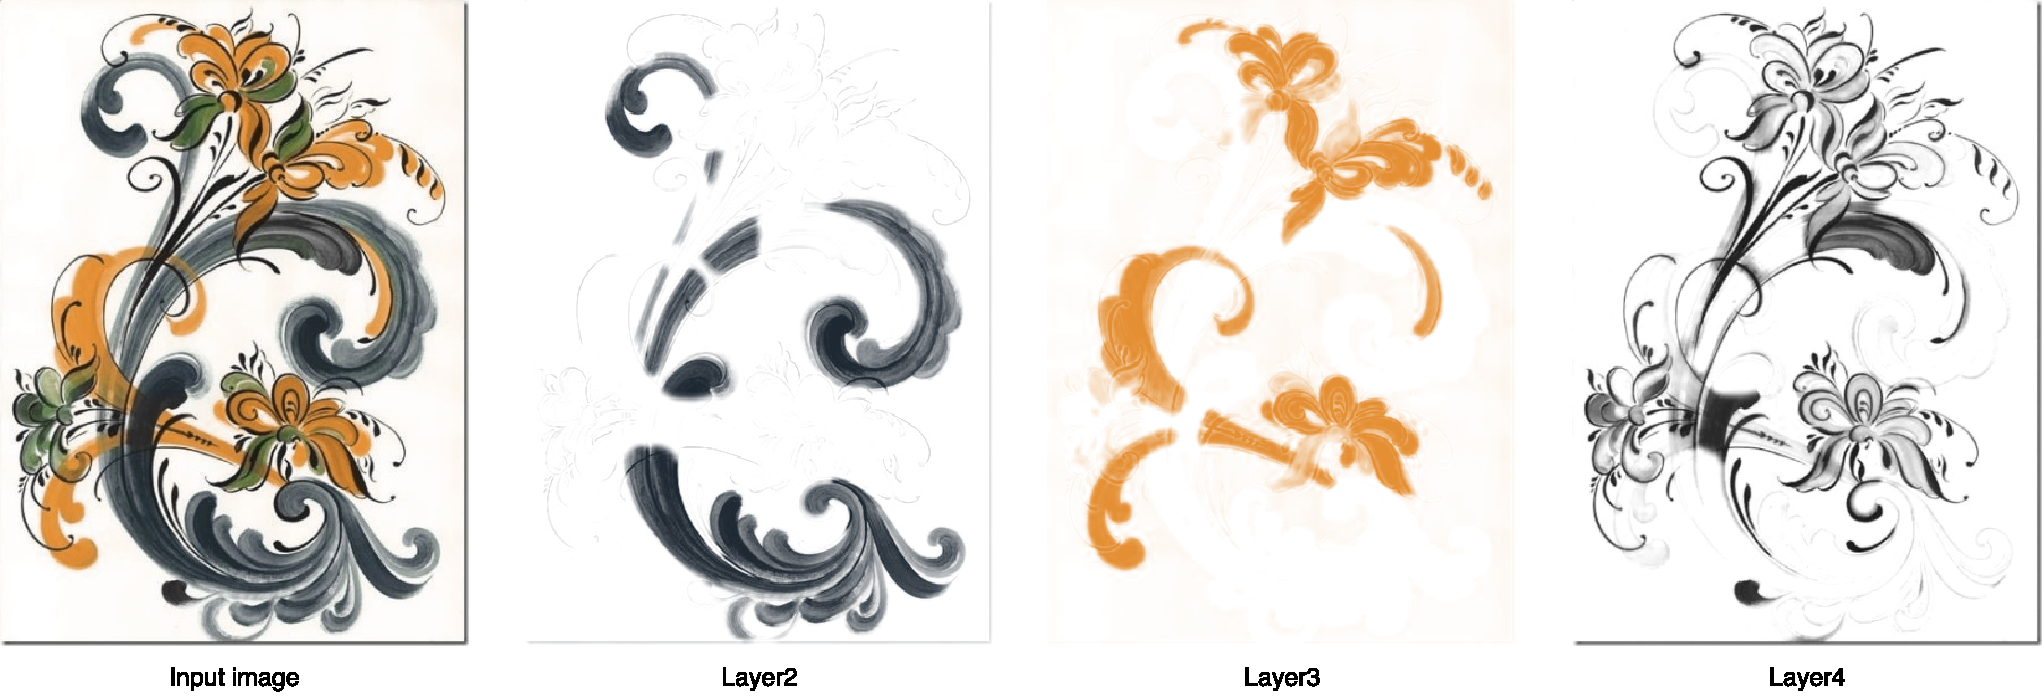
\includegraphics[height=0.2\textheight]{layers.pdf}
\caption{Decomposition layers }
\label{decom:4layers}
\end{figure}
As shown in Figure \ref{decom:4layers}, a given painting is firstly decomposed into a set of layers in terms of RGB values. Secondly, each resulting layer is further segmented into multiple regions which represent brush strokes respectively. Thirdly, the depth map of each brush stroke is generated by the shape from shading technique	s individually. After that, the desired bas-relief is generated by merging all the depth maps of brush strokes together.
\newline
The key point is to extract brush strokes from input paintings. Overlapped strokes make colors blend. To deal with it, layer decomposition is firstly employed here, which decomposes the painting into a set of single colored and translucent layers. In brush paintings, each stroke only utilizes a single palette color. Therefore, layer decomposition helps classify brush strokes separately into different layers based on the palette color so that every layer contains the strokes which are well separated.
However, wrong layer decomposition may cut one stroke into two or more layers. It is observed that typically strokes of such paintings follow regular patterns. For instance, Rosemaling paintings employ many C and S strokes, and the color and transparency change very little in the direction of the stroke. We introduce the edge tangent flow (ETF) field and the coherent line \cite{kang2007coherent} to enhance such features in paintings, which is in favor of preserving the wholeness of the strokes in every layer and effectively avoid wrong layer decomposition.
\newline
The coherent line is further involved in the MSERs algorithm \cite{donoser2006efficient} again for extracting spurious edges within one layer.
Furthermore, to generate the depth maps of the strokes individually, we perform shape from shading on the opacity of the paintings instead of the intensity her	e, since the opacity has a bigger range than the intensity (as can be seen in Figure \ref{histo} for detail). SFS techniques may generate details of surfaces in terms of image texture. It is desirable to transfer the features of the paintings, e.g. the density of colors, to the surface of the brush stroke models.
\newline
The depth maps of all the strokes are then merged together to form the desired bas-relief. We hope to point out that the employed orthographic SFS technique tends to encourage interior growth within a closed region due to the Eikonal Equation, which may result in the growth of a background region surrounded by strokes. In general, the background plane should be unchanged. Thus, generating strokes individually not only benefits the composition of bas-reliefs but also avoid this technique issue.
Moreover, the stroke order and shape may be edited by users to cater for the request of recomposition in art design. The user may recompose the stroke models in 3D space for secondary creation.
\newpage 
\newpage  \chapter{LAYER DECOMPOSITION}
Digital painting with different layers is an integral feature of digital image editing software. However, layers may never have existed for a scanned physical painting.Layers offer an intuitive way to edit the color and geometry of components and localize changes to the desired portion of the final image. Without layers, brush stroke segmentation becomes extremely challenging, since they can overlap and blend with each other.So,before extracting brush strokes, we decompose a Chinese painting into layers.\\
In our decomposition, each layer represents one coat of a painting with single color that is applied with varying opacity throughout the input painting. Wrong layer decomposition may cut one stroke into different layers. It is crucial to preserve the completeness and smoothness of the brush strokes in layer decomposition. To this end, we modify the layer decomposition algorithm in \cite{tan2016decomposing} by involving the coherent lines \cite{kang2007coherent} in our implementation. In the following we first address the layer decomposition algorithm \cite{tan2016decomposing} briefly and then discuss our modification. 


\section{Identify Paint Colors}

\begin{figure}[H]
	\centering
	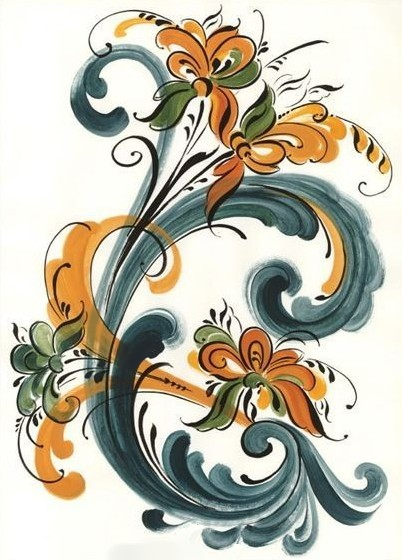
\includegraphics[height=0.2\textheight]{5.png}
	~~~~
	\includegraphics[height=0.2\textheight]{cube1.png}
	\caption{Geometry of input image pixels in RGB-space}
	\label{point cloud}
\end{figure}

In a brush painting, one region may have been painted multiply time with different paint colors. We assume that the color on each pixel is a linear combination of the paint colors, so all the pixel color in the input painting lies the convex hull of in the RGB space as showed in Figure \ref{point cloud} and Figure \ref{convex} , and every vertice is considered as a paint color. And base on such idea, we can represent each pixel color based on painted colors: 
\begin{equation*}
p=\Sigma \omega_i c_i
\end{equation*}
$p$ represents the color of the pixel, and $c_i$ represents the $i$-th paint color. 
To compute the paint color, we introduced the convex hull simplifying method of Tan's work \cite{tan2016decomposing}. In which a convex hull of the colors in RGB space should be computed, while every vertice is considered as a paint color. The colors would be tightly wrapped by the convex hull, but normally there would be many vertices more than what we need, since too many vertices would result in too many layers. In Tan's work \cite{tan2016decomposing} they provide a simplification method which would output manageable number of layers based on user need and the output layers with clearly differentiated colors,as showed in Figure \ref{convex}. And based on such method ,we generate a palette of paint colors of the input paintings. 

\begin{figure}[H]
	\centering
	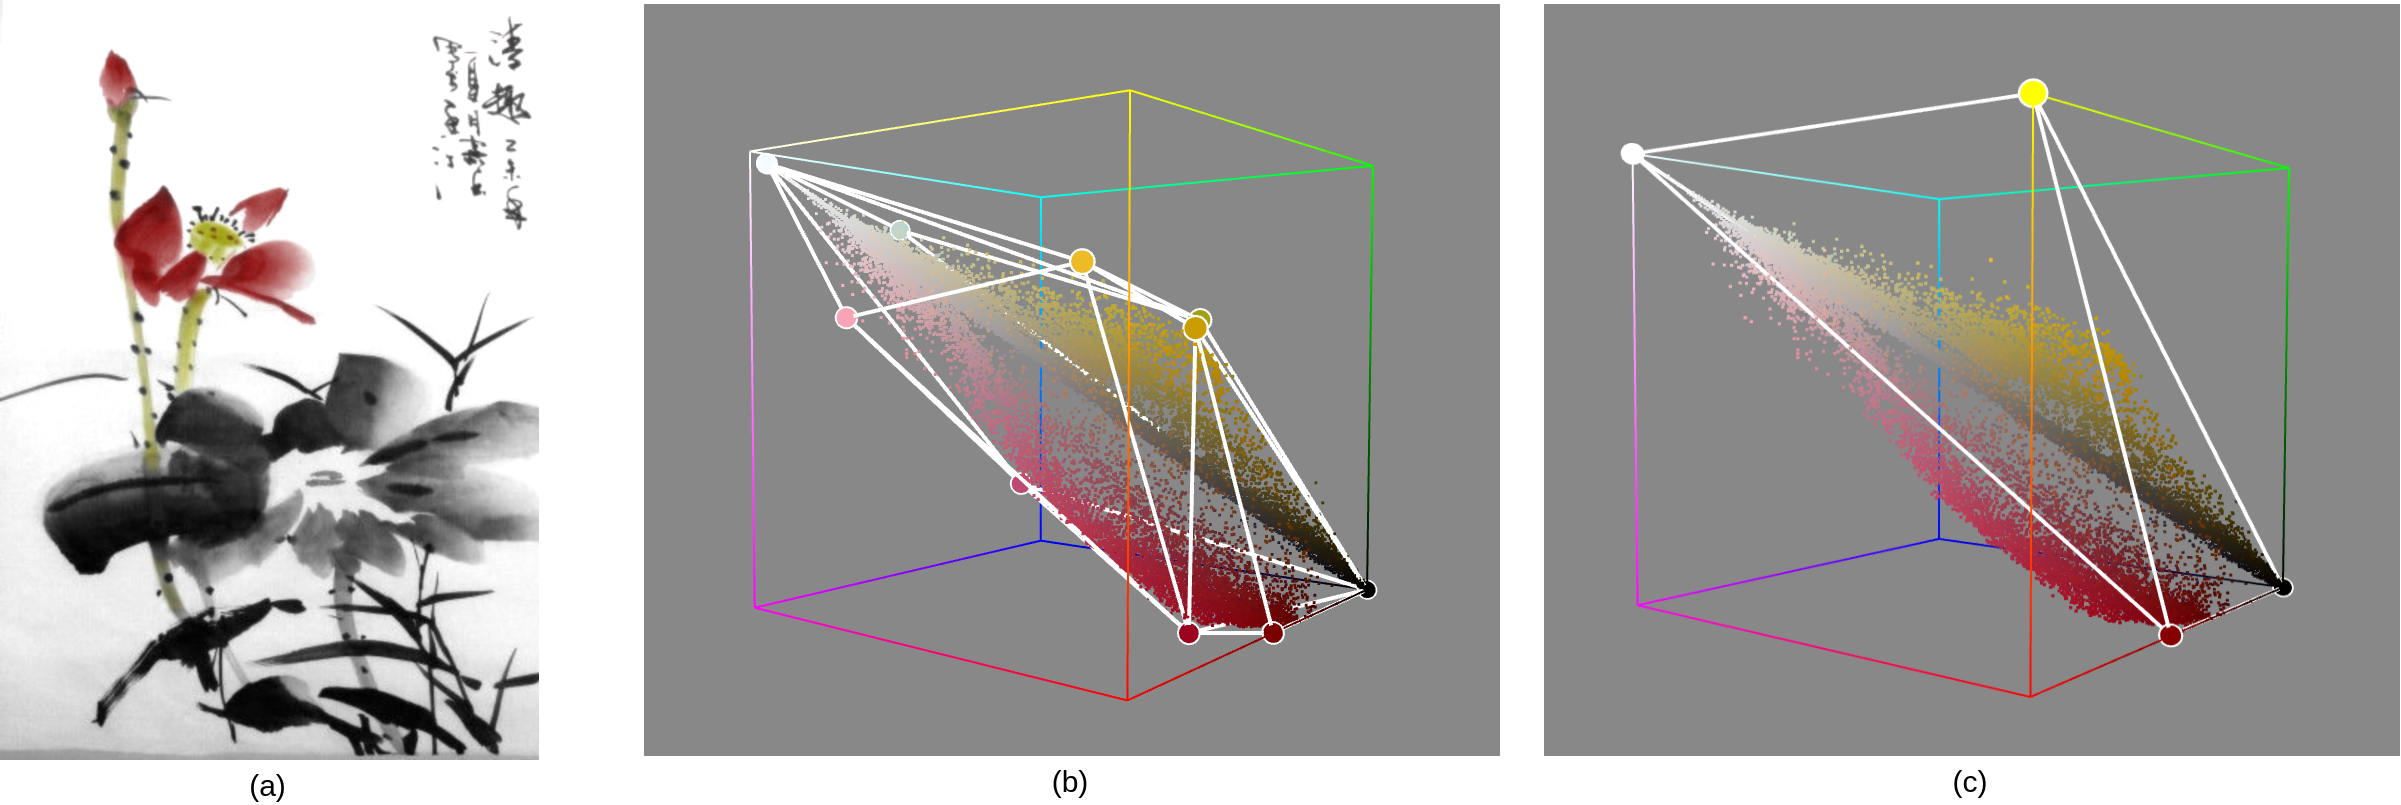
\includegraphics[height=0.18\textheight]{convex.png}
	\caption{Convex hull of input image}
	\label{convex}
	\medskip
	\small
	(a) A simple digital painting’s (b) convex hull in RGB-space is complex due to rounding. (c) The result of simplification algorithm 
\end{figure}

\section{Layer Decomposition Scheme}

\begin{figure}[H]
	\centering
	\includegraphics[height=0.2\textheight]{Layers.png}
	\caption{Decomposition layers }
	\label{decom:4layers}
\end{figure}

The standard Porter-Duff “A over B” compositing operation in \cite{porter1984compositing} is described that when the pixel $A$ with color $A_{RGB}$ and translucency $\alpha_{A}$ is placed over the pixel $B$ with color $B_{RGB}$ and translucency $\alpha_{B}$, the observed color is, 
\[  \left ( \frac{A}{B} \right )_{RGB}=\frac{\alpha_{A}A_{RGB}-(1-\alpha_{A})\alpha_{B}B_{RGB}}{\left ( \frac{A}{B} \right )_{\alpha}} \]
where 
\[\left ( \frac{A}{B} \right )_{\alpha} = \alpha_{A}+(1-\alpha_{A})\alpha_{B} \] 
Each pixel’s color is viewed as the convex combination of all layers’ colors. For each pixel, the observed color p can be approximated by the recursive application of the compositing. We take as input ordered RGB layer colors through computing per-pixel opacity values for each layer. The following ‘polynomial’ regularization term penalizes the difference between the observed color p and the polynomial approximation based on the “A over B” compositing \cite{porter1984compositing},

\[E_{polynomial}=\frac{1}{K}\left \|    C_{n}+\sum_{i=1}^{n}  \left ( \left ( C_{i-1}-C_{i} \right ) \prod_{j=i}^{n}(1-\alpha_{j}) \right )-p  \right \|^{2}\]

where $C_{i}$ denotes the i-th layer’s color, is the opacity of $\alpha_{i}$ , the background color $C_{i}$ is opaque, $K=3$ and or 4 depending on the number of channels $(RGB$ or $RGB-\alpha)$. The opacity penalty is expressed as,
\[E_{opaque}=\frac{1}{n}\sum_{i=1}^n-(1-\alpha_{i})^2\]
The default smoothness penalty is expressed as,

\[E_{spatial}=\frac{1}{n}\sum_{i=1}^n( \bigtriangledown  \alpha_{i})^2\]

where $ \bigtriangledown  \alpha_{i}$is the spatial gradient of opacity in the i-th layer. This term penalizes solutions which are not spatially smooth. However, the gradient of opacity is not always aligned with that of intensity, which may result in edges discontinuous.
The users may specify the layer order in advance, as well as the number of layers, n, is given. The opacity for every layer may be solved by minimizing the following combined cost function,
\begin{equation}
E=\omega_{polynomial}E_{polynomial}+\omega_{opaque}E_{opaque}+\omega_{spatial}E_{spatial}
\label{eq:layer1}
\end{equation} 
where $\omega_{polynomial} = 375 ,\omega_{opaque}=1 , \omega_{spatial}=10$. 

\subsection{Our Modified Layer Decomposition}
\begin{figure}[H]
	\centering
	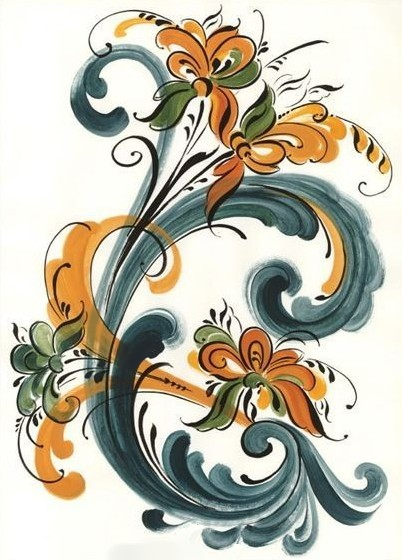
\includegraphics[width=4cm]{5.png}
	~~~~
	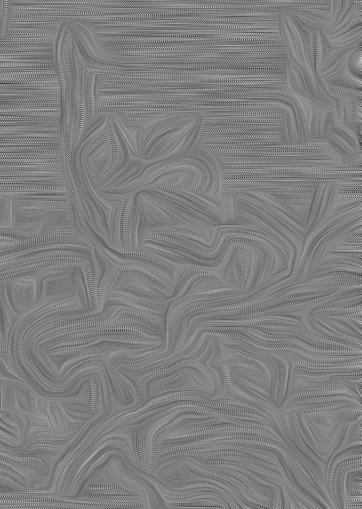
\includegraphics[width=4cm]{5etf.png}
	\caption{Edge Tangent Flow}
	\label{ETF}
\end{figure}

As we can see in Figure \ref{decom:4layers},the extracted layers failed to maintain the completeness of the brush strokes, especially in the first layer. To enhance the smoothness and completeness of extracted strokes, the coherent line drawing technique in \cite{kang2007coherent} is introduced to Eq \ref{eq:layer1} ,which is a flow-guided anisotropic filtering framework.In the coherent line drawing technique, the edge tangent flow(ETF) of a image is calculated, represented by a vector $t^{new(x)} $. Here, we use vector $t^{new(x)} $ to mimic the brush stroke direction.  Figure \ref{ETF} shows the edge tangent flow $($ETF$)$ field of a Chinese painting.\newline
The ETF field is defined as,
\begin{equation}
 t^{new(x)}=\frac{1}{k}\sum_{y\in\Omega(x)} \varphi(x,y)t^{current}(y)\omega_{s}(x,y)\omega_{m}(x,y)\omega_{d}(x,y)
 \label{eq:layer_etf} 
\end{equation}

$t(x)$ denotes the normalized tangent vector at pixel $x$, $\Omega(x)$ denotes the neighborhood of the pixel $x$, and $k$ is the term of vector normalization. The spatial weight function $\omega_{s}$ employs the radially-symmetric box filter with some radius. The magnitude weight function $\omega_{m}$ is monotonically increasing, indicating that the bigger weights are given to the neighboring pixels y whose gradient magnitudes are higher than that of the central pixel x. This ensures the preservation of the dominant edge directions. The direction weight function, $\omega_{d}$, may enhance alignment of vectors, e.g. $t(x)\cdot t(y)>0$ , while suppressing swirling flows. In addition, the sign function $\varphi(x,y)$  is employed to prevent the swirling artifact as well.

\begin{figure}[H]
	\centering
	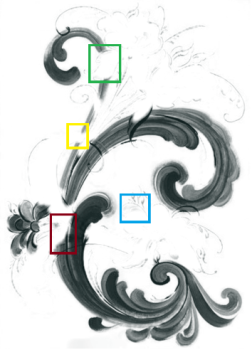
\includegraphics[width=5cm]{com_layer1.png}
	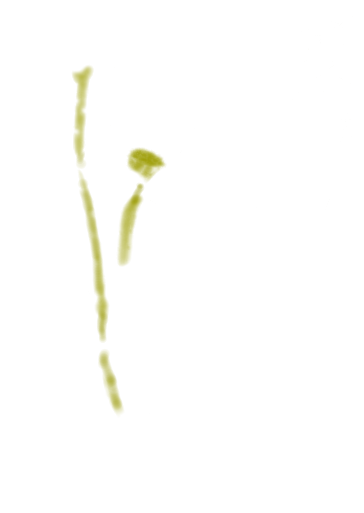
\includegraphics[width=5cm]{com_layer2.png}
	\caption{Comparison of layer decomposition  }
	\label{com eflow}
	\medskip
	\small
	Comparison of decomposed first layer before and after modification. Left shows the original result of Eq \ref{eq:layer1} , right shows the result by using $E_{flow}$ instead of $E_{spatial}$ in Eq \ref{eq:layer1}.
\end{figure}

Involving ETF filed of Eq \ref{eq:layer_etf} in $E_{spatial}$, the smoothness penalty is rewritten as,

\begin{equation} 
E_{flow}=\frac{1}{n} \sum_{i=1}^{n} \left \| t^{new} \right \| \left ( \bigtriangledown_{\theta}\alpha_{i} \right )^2 
\end{equation} 

where $\theta$ denotes the direction of $t^{new}$, and $ \bigtriangledown_{\theta}\alpha_{i} $ is the gradient of opacity in the direction of $t^{new}$. Moreover, we weight this penalty by the norm of $t^{new}$. Applying the updated $E_{flow}$ to the layer decomposition of Eq \ref{eq:layer1} instead of $E_{spatial}$, the strokes become complete and smooth, which can be noted in Figure \ref{com eflow}.

\begin{figure}[H]
	\centering
	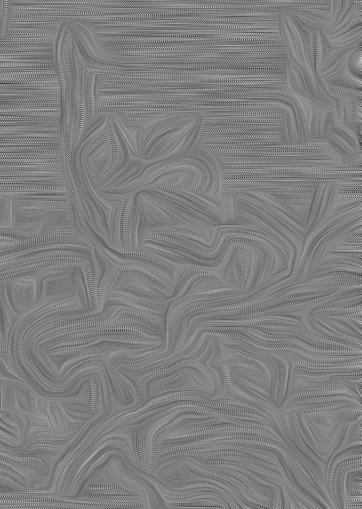
\includegraphics[width=5cm]{5etf.png}
	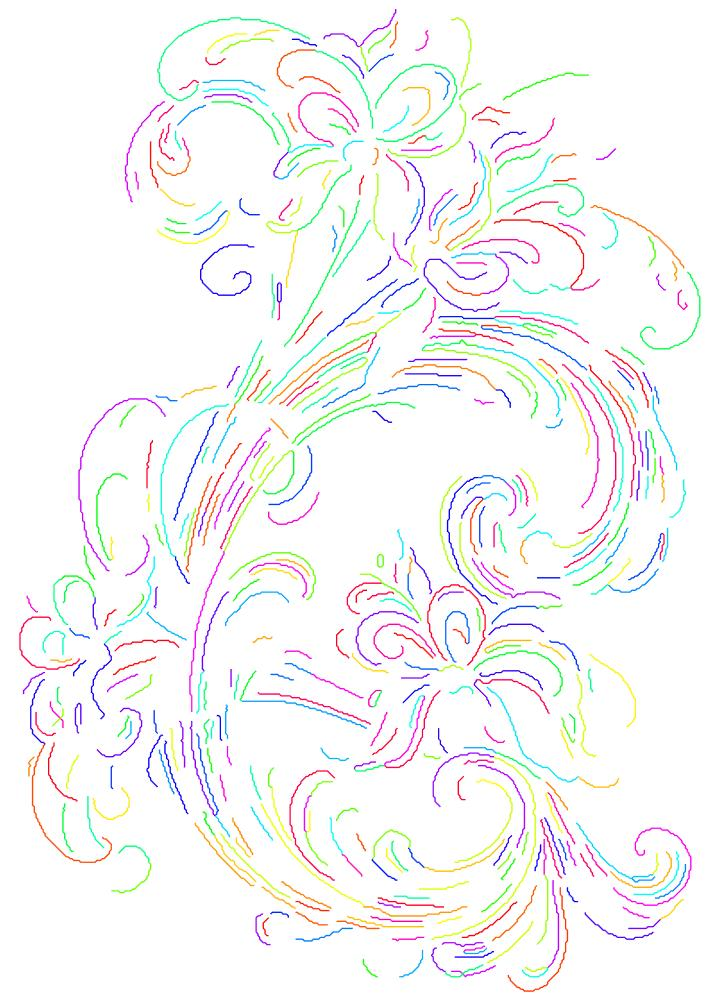
\includegraphics[width=5cm]{edge.png}
	\caption{Edge Tangent Flow field and coherent lines of the painting.}
\end{figure}


Second, the coherent lines as the constraint of brush stroke edges are involved in layer decomposition of Eq \ref{eq:layer1}. Herein, the coherent lines can be computed as follows.
\begin{figure}[H]
	\centering
	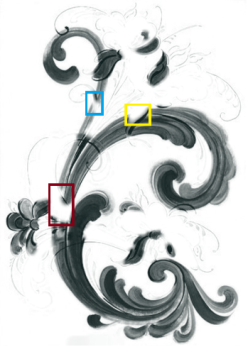
\includegraphics[width=5cm]{com_layer3.png}
	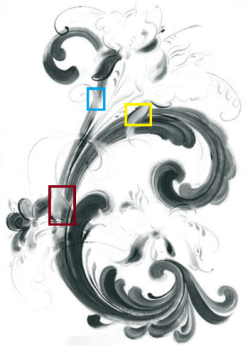
\includegraphics[width=5cm]{com_layer4.png}
	\caption{Comparison of layer decomposition before and after using $E_{egde}$  in Eq \ref{eq:layer1}; }
	\label{com:edge}
\end{figure}
Given a ETF field $t(x)$, the flow-guided anisotropic Difference of Gaussian (DoG) filter is employed, in which the kernel shape is defined by the local flow encoded in ETF field. Note that $t(x)$ represents the local edge direction. It is most likely to make the highest contrast in the perpendicular direction, that is, the gradient direction. When moving along the edge flow, the DoG filter is applied in the gradient direction. As a result, we can ‘exaggerate’ the filter output along genuine edges, while ‘attenuating’ the output from spurious edges. This not only enhances the coherence of the edges, but also suppresses noises. Iteratively applying this flow-based DoG filter results in a binary output which reaches a satisfactory level of line connectivity and illustration quality. The coherent lines can be regarded as the edges of brush strokes.

\begin{figure}[H]
 		\centering
	\begin{subfigure}[b]{0.4\textwidth}
		\centering
		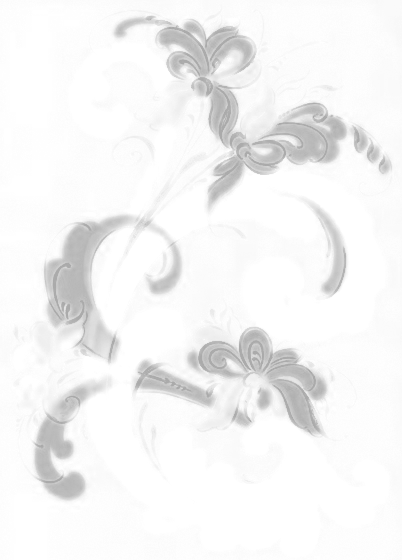
\includegraphics[width=\textwidth]{intensity.png}
		\caption{intensity map of layer2}
	\end{subfigure}
	~
	\begin{subfigure}[b]{0.4\textwidth}
		\centering
		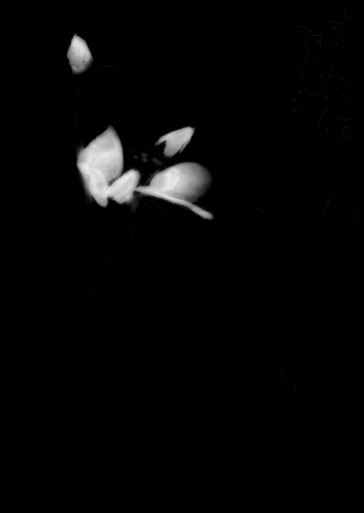
\includegraphics[width=\textwidth]{alpha.png}
		\caption{alpha map of layer2}
	\end{subfigure}
 

 
	\centering
	\begin{subfigure}[b]{0.4\textwidth}
		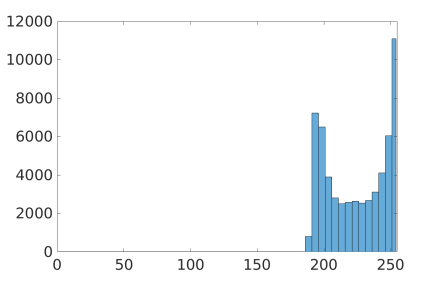
\includegraphics[clip,width=\textwidth]{h1.png}
		\caption{histogram of intensity map of layer2}
	\end{subfigure}
	~  	
	\begin{subfigure}[b]{0.4\textwidth}
		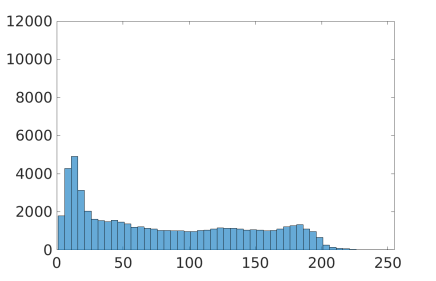
\includegraphics[clip,width=\textwidth]{h2.png}
		\caption{histogram of alpha map of layer2}
	\end{subfigure}
	\caption{Comparison between transparency and intensity of layer2}
	\label{histo}
\end{figure}



 
To preserve the stroke edges, we assume that the opacity along the coherent lines is consistent, i.e. $min \int_{l}\Arrowvert \bigtriangledown\alpha \Arrowvert^2 dx $, where l denotes the collection of coherent lines. Hence, the constraint term is defined by applying Laplacian operator to the opacity along the coherent lines,

\begin{equation} 
E_{edge}=\Arrowvert LY \Arrowvert^2 
\end{equation} 

where all the opacity $\alpha_i$ are stacked in the vector $Y$, and $L$ denotes the connection matrix. The eight-connected neighboring rule is utilized to construct the connection matrix $L$, that is, if two adjacent pixels, i and j, stay on the same coherent line, the item of $L(i,j)$ is set to -1 ; otherwise 0. Figure \ref{com:edge}a and \ref{com:edge}b shows that the edges of strokes become visible and complete after involving $E_{edge}$ into Eq \ref{eq:layer1}.
Accordingly, the layer decomposition of Eq \ref{eq:layer1} is rewritten as,

\begin{equation}
E=\omega_{polynomial}E_{polynomial}+\omega_{opaque}E_{opaque}+\omega_{flow}E_{flow}+\omega_{edge}E_{edge}
\label{eq:layer_sum}
\end{equation} 

where $\omega_{flow}=100, \omega_{edge}=20 $ for all our examples. Figure 8 shows an evaluation of the effect of changing weights.

To demonstrate our results can better preserve the smoothness and completeness of brush strokes, we perform the schemes of Eq \ref{eq:layer1} and Eq \ref{eq:layer_sum} separately on the same set of Chinese paintings and compare the root-mean-square-error (RMSE) of the opacity of the coherent lines on each layer shown in Table 1. The RMSE by Eq \ref{eq:layer_sum} is noticeably less than that by Eq \ref{eq:layer1}. This means that the coherent lines have been embedded into the opacity of each layer. The weights are empirically determined in terms of the opacity RMSE of coherent lines. \\
To demonstrate the robustness of our approach, including Chinese paintings, we also perform the comparison on some other paintings with highly characteristic brush strokes, such as rosemailing paintings\cite{ellingsgard1978rosemaling} and Vincent van Gogh's paintings\cite{li2012rhythmic}.

\begin{figure}
	\centering
	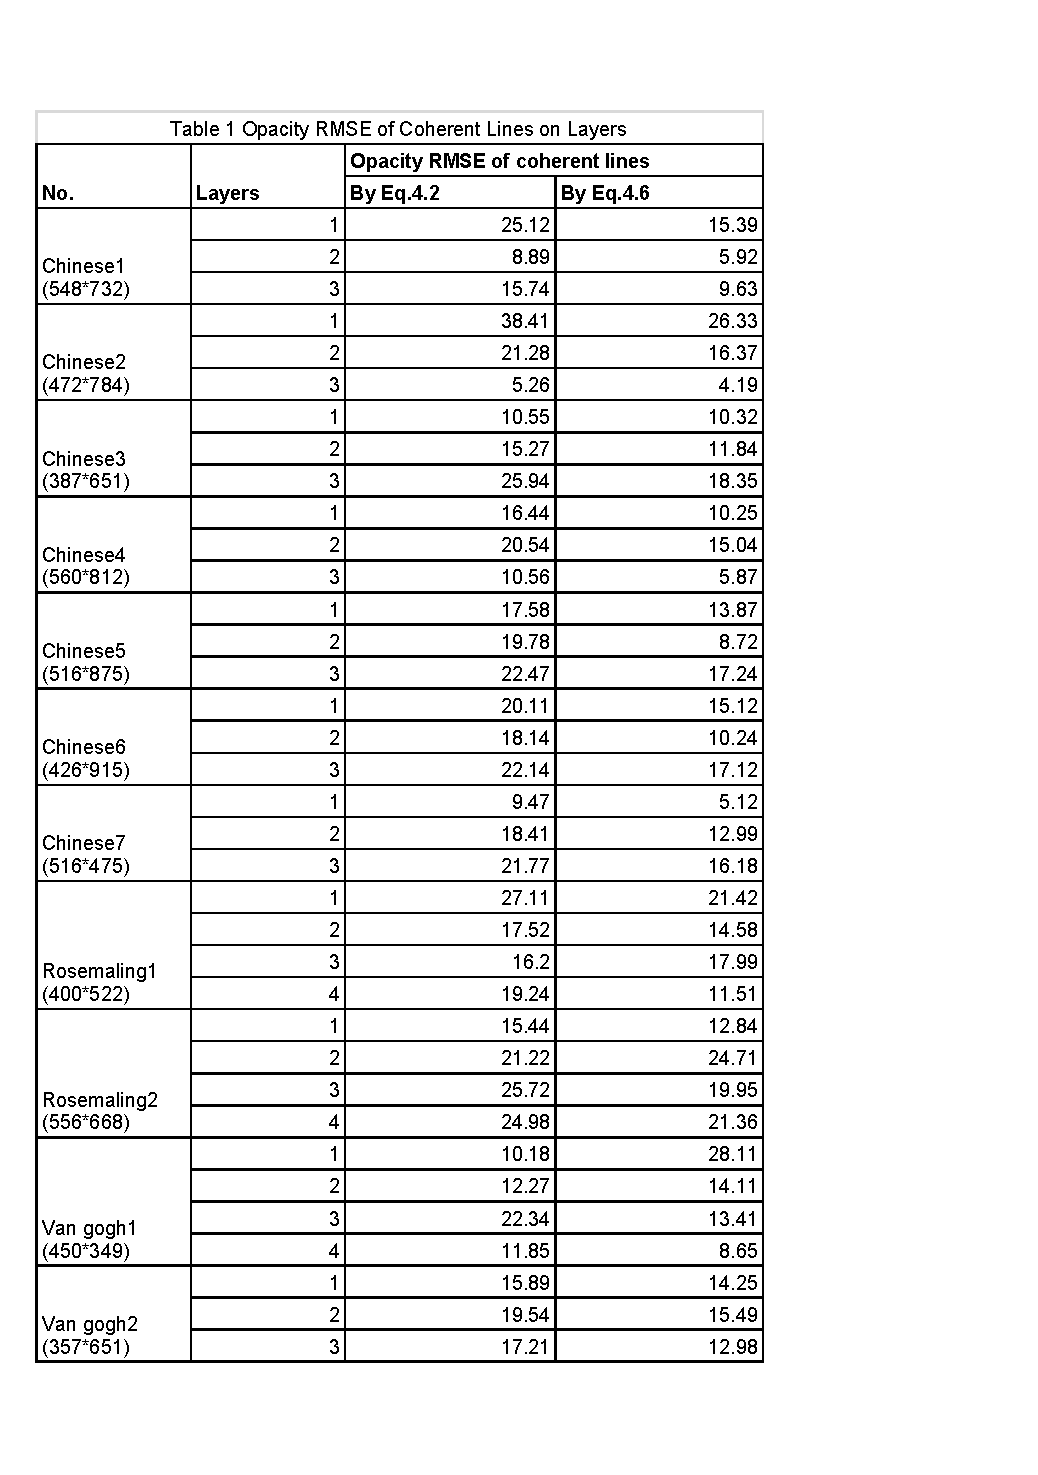
\includegraphics[width=17cm]{rmse.pdf}

\end{figure}


















\newpage  \clearpage
\chapter{EXTRACTION OF BRUSH STROKES}\label{extract}
To generated bas-relief model from brush strokes,we need to first extract brush strokes.In this chapter, we demonstrate how to extract brush strokes from decomposed layers by using modified Maximally Stable Extremal Regions (MSERs) algorithm, and we show that our optimization is more suitable for brush stroke extraction. In this chapter, the default MSERs algorithm \cite{donoser2006efficient} and our modified algorithm are explained and their main characteristics compared. By successfully extract brush strokes, our algorithm can also be used in image editing,see section \ref{editing}.\\
The Maximally Stable Extremal Regions (MSERs) algorithm proposed in \cite{donoser2006efficient} is used for feature detection and image segmentation. A MSER is a 2D region detected by MSERs algorithm.  Generally,a brush stroke is considered as a closed stable region on paintings and it might be painted on different scales. MSERs have properties that form their superior performance as stable segmentation. The segmented MSER is closed under continuous geometric transformations and is invariant to affine intensity changes. Furthermore MSER are detected at different scales. So, we employ the Maximally Stable Extremal Regions (MSERs) proposed in \cite{donoser2006efficient} to extract brush strokes. MSERs algorithm requires a distinct difference between background and foreground while allowing a small variation of intensity within the selected stroke region. Usually, the brush strokes on the decomposed layers satisfy this requirement.
However, MSERs may fail in segmentation with the following scenarios,\\ 
(1) The brush stroke with the intensity very close to the background; \\
(2) Two adjacent brush stroke painted by different colors with the similar intensity;\\
(3) Overlapped brush strokes.\\
(4) Moreover, like the other existing segmentation approaches, the MSERs algorithm encounters over-segmentation issue as well. \\
To tackle these challenges, the coherent lines \cite{kang2007coherent} is introduced into MSERs, which both enhances the edges of strokes and preserves the completeness of strokes. For completeness sake, we briefly address MSERs algorithm and then address our modification.
\section{MSERs Algorithm}

\begin{figure}[H] \label{defumser}
	\centering
	\begin{subfigure}[b]{0.4\textwidth}
		\centering
		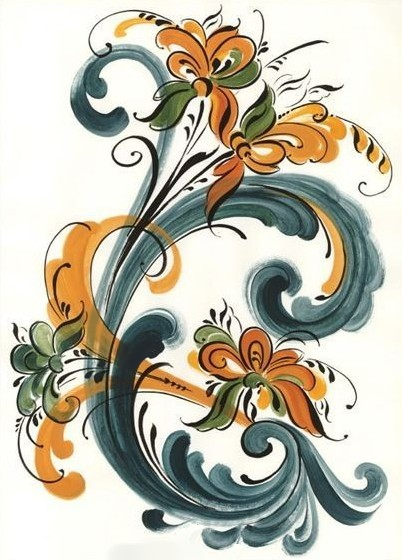
\includegraphics[width=\textwidth]{5.png}
		\caption{input image}
	\end{subfigure}
	~  
	\begin{subfigure}[b]{0.4\textwidth} 
		\centering
		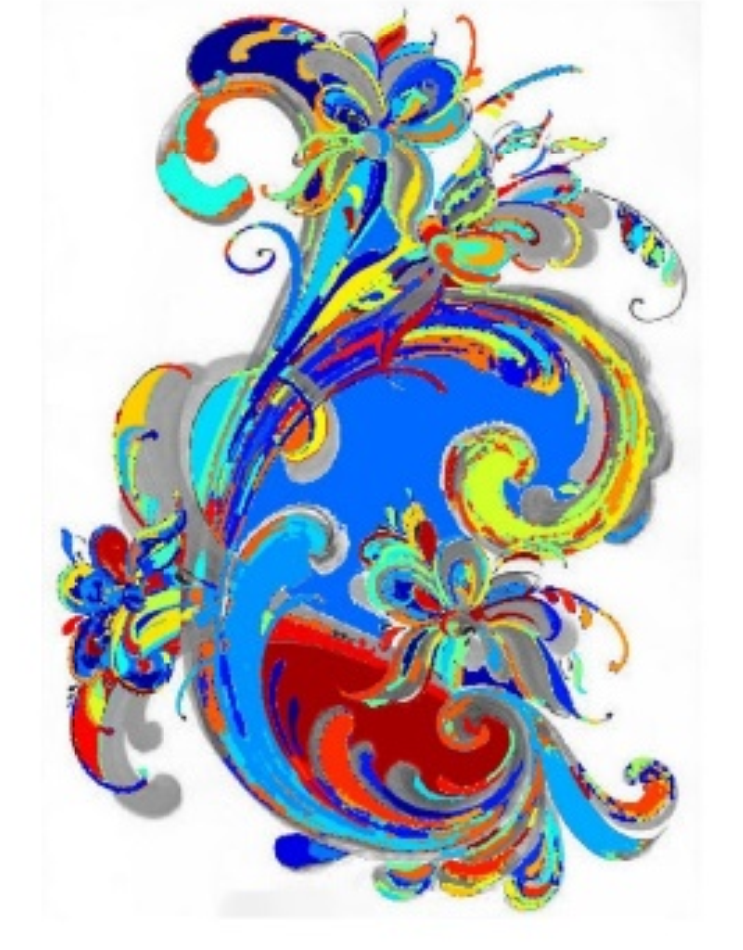
\includegraphics[width=\textwidth]{inten_mser.png}
		\caption{MSERs of the input image}	
	\end{subfigure}

	
	Perform the original MSERs on the intensity of image,different color(except black) indicates different regions.
\end{figure}


MSERs can denote a set of distinguished regions that are detected in an intensity image. All of these regions are defined by an extremal property of the intensity function in the region and on its outer boundary, i.e. for a given extremal region S, the internal intensity is more than the intensity of boundary of S,

\[ \forall p \in S,\forall q \in \partial S , \longrightarrow I(p) \geq I(q)\]

where $\partial S $ denotes the boundary of $S$.$p$ and $q$ represent different pixels on the image, and $I(x)$ represent the intensity value of pixel $x$. 
Changing threshold, the extremal regions may further split or merge. The resulting extremal regions may be represented by the component tree. Accordingly, we may compute the change rate of the area of extremal region by

\[ \gamma(S_i^g) = \frac{\left ( \left |  S_j^{g-\Delta} \right |-\left |  S_k^{g+\Delta} \right | \right )}{\arrowvert S_i^g\arrowvert} \]

where $ \left | .  \right |$  denotes the cardinality, $ S_{i}^{g} $  is the i-th region which is obtained by thresholding at an intensity value g and $\Delta $ is a stability range parameter. $  g-\Delta $ and $ g+\Delta $ are obtained by moving upward and downward respectively in the component tree from the region $ S_{i} $ until a region with intensity value   or  is found. $ \left \{ i,j,k \right \}$ are the indices of nodes of the component tree. MSERs correspond to those nodes of the component tree that have a stability value $\gamma$, which is a local minimum along the path to the root of the tree.


\section{Modified MSERs Algorithm}\label{modimesr}

In terms of the definition of the area change rate $ \gamma $, the default MSERs algorithm may fail in segmentation with the following scenarios,\\
(1) The brush stroke with the intensity very close to the background; \\
(2) Adjacent brush strokes painted by different colors with the similar intensity;\\
(3) Overlapped brush strokes with different color.\\ 
(4) Moreover, like the other existing segmentation approaches, the MSERs algorithm encounters over-segmentation issue as well. \\
Comparing with default MSERs algorithm use intensity of input, our extraction is performed on opacity of generated layers.By doing so,in each layer, the opacity of the background is close to zero, which can be easily filter out, see Figure \ref{mser:alpha} , so, the first scenario can be handled. \\
The opacity of the brush strokes is always independent of the color,so two adjacent brush stroke painted by different colors would be separated into different layers, so,naturally,our extraction is suitable for the second scenario and third scenario, see Figure \ref{mser:alpha}. \\
Moreover, we perform the layer decomposition of Eq \ref{eq:layer_sum} on a brush painting and show the intensity and opacity of one layer associated with the individual histograms in Figure \ref{histo}. It can be noted that the opacity of the layer contains richer layered details than the intensity. So,our first modification is to perform MSERs on the opacity of every layer.\\
Secondly,we aim at the third scenarios of over-segmentation. When the extremal region is growing up through changing threshold, it is feasible to restrict the region by introducing the coherent lines. According to the definition of the extremal region, the boundary of region $S$ should satisfy,

\begin{equation*}
 \forall p \in S,\forall z \in   \bar{S} , \forall q \in \partial S \longrightarrow I(p) \geq I(q)  ~\mathrm{and}~  I(q) \leq I(z)
\end{equation*}
 
where $ \bar{S} $ denotes the complement of $S$. The second modification is to simply modify the opacity of layers, that is, overlapping the coherent lines with the layer and then changing the opacity of coherent lines to the smallest value in the layer.

To deal with the over-segmentation issue, the coherent lines play an important role. Given a region $S$, we modify the area change rate $\gamma$ as,
\begin{equation}
\gamma(S_i^g)=\frac{  \lvert \lvert S_j^{g-\Delta}\rvert -\lvert S_k^{g+\Delta} \rvert
	 \rvert     }{\arrowvert S_i^g\arrowvert} + \frac{  \lvert \lvert Q_j^{g-\Delta}\rvert -\lvert Q_k^{g+\Delta} \rvert
	 \rvert     }{\arrowvert Q_i^g\arrowvert} - (1-\frac{\lvert Q_i\rvert}{\lvert \partial S_i^g \rvert} )
\end{equation}


where $Q$ denotes the set of pixels which stay on the coherent lines and $Q \subset \partial S $. The third modification is to take into account the change of coherent lines to the boundary of $S$, i.e. the third term penalizes that a small portion of the boundary $\partial S$ is occupied by coherent lines.

Figure \ref{mser:alpha} shows the segmentation results by the modified MSERs, which correspond to brush strokes. It can be noted that performing MSERs on the intensity of image inevitable yields over-segmentations. Performing the modified MSERs on the opacity of layers, the strokes tend to complete and smooth within one layer. Moreover, some small regions with the distinct opacity values against neighboring areas have been filtered out, and no region is selected from background. 
\begin{figure}[H]
	\centering 
	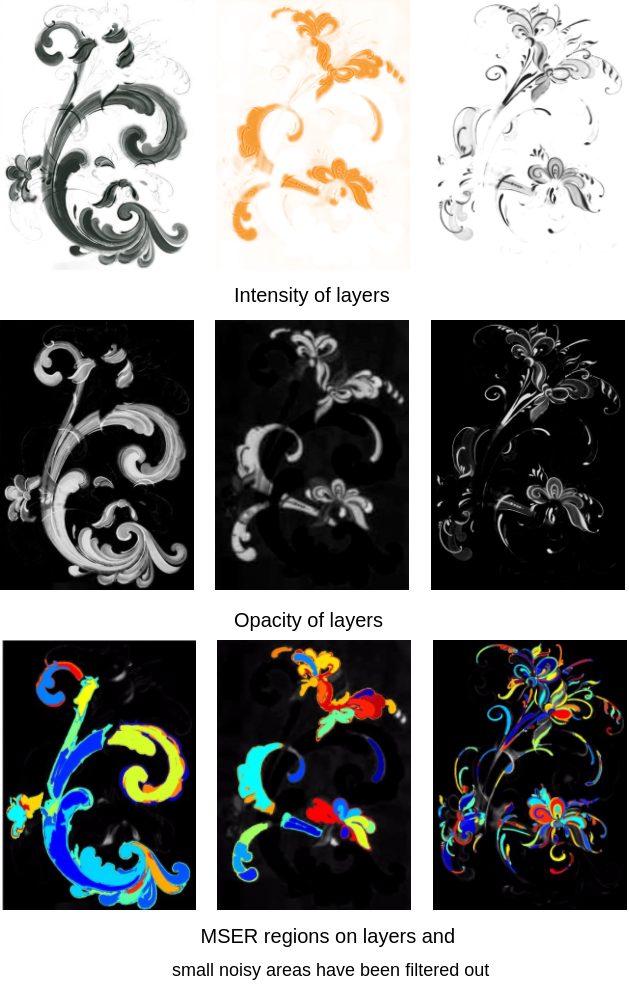
\includegraphics[width=10cm]{layer_sum.png}
	\caption{The opacity maps, and MSER regions of three layers by the modified MSERs.}
	\label{mser:alpha}
\end{figure}

\section{Comparison and Evaluation of Brush Stroke Extraction} \label{comparevan}
To the best of our knowledge, there is lack of study on automatic brush strokes extraction. Li et al.\cite{li2012rhythmic} present a automatic brush stroke extraction method based on seed growing. To numerically evaluate their brush stroke extraction algorithm, they generated manually marked brush strokes using 10 example regions from van Gogh's paintings, see Figure \ref{liswork}. \\ 
Based on the manually marked examples, they define two parameters which can be measured in order to evaluate the accuracy of extracted brush stroke and,therefore, can be used to compare between their method and ours: valid rate and detection rate.\\
Valid rate:the percentage of valid automatically extracted brush strokes. \\ Detection rate: The percentage of detected manual brush strokes . \\
Even through our brush stroke extraction algorithm is not designed specifically for van Gogh's paintings, for fair comparison, we use the van Gogh's painting given in their research, as shown in Figure \ref{vanourwork}.\\
As shown in Table 2,the valid rate and detection rate of our method is noticeably higher than Li et al.'s method \cite{li2012rhythmic} (The paint ID is given by Li et al.'s work). 
\begin{figure}[H]
	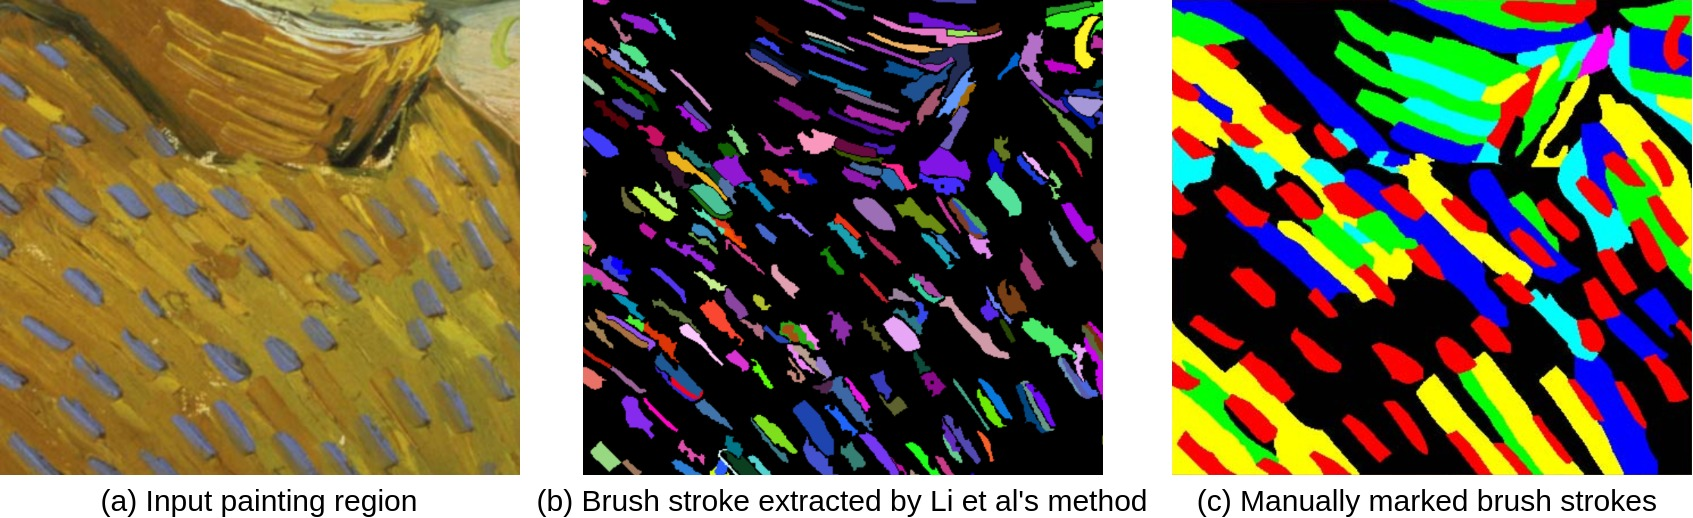
\includegraphics[width=14cm]{strokecompare.jpg}
	\caption{Brush strokes extraction in Li et al.'s work}
	\label{liswork}
\end{figure}
\begin{figure}[H]
	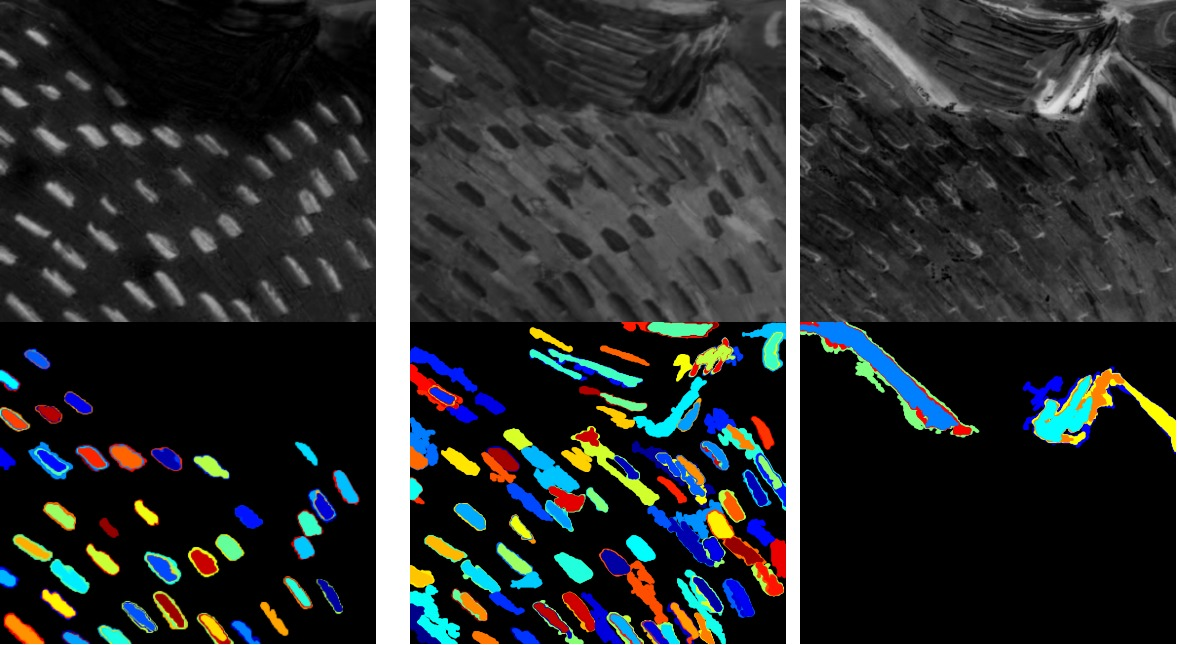
\includegraphics[width=14cm]{strokecompare1.jpg}
	\caption{Brush strokes extraction by our method}
	\label{vanourwork}
\end{figure}


\begin{figure}[H]
	\includegraphics[width=14cm]{comstroke.pdf}
	\label{table2}
\end{figure}
As shown in Table 2, our method extracts brush strokes with higher accuracy.





\section{Image editing based on brush strokes}\label{editing}

Once the brushstrokes are extracted,we can simply recoloring strokes by assign a RGB value to the brushstroke while keep its opacity value.
Figure \ref{recoloring} a and \ref{recoloring} b shows recoloring strokes on three paintings respectively. As the strokes have been extracted, it is easy to separately recolor one or more strokes with different colors. 

Figure \ref{recoloring} c shows stroke manipulation through inserting objects . One of image editing tasks is to change a specified region with a new object in a seamless and effortless manner. Here we are interested in inserting new objects into a painting while keeping the transparency of the painting. Note that the inserted objects are opaque and are inserted between  brush strokes here. The occluded regions of the objects are visible due to the transparency of the brush strokes. Unlike the traditional image synthesis approaches, our implementation works on the strokes, which both guarantees seamless and keep the transparency of brush strokes on the painting.


\begin{figure}[H]
	\centering
	\includegraphics[width=15cm]{recoloring.png}
	\caption{Image editing based on brush strokes}
	\label{recoloring}
	\medskip
Column a) shows 3 kinds of brush paintings, Chinese painting ,Rosemailing,and van Gogh oil painting . Column b) shows recoloring multiple strokes. Herein, for van Gogh oil painting, we show recoloring all the brushstrokes in one layer. Column c) shows inserting objects into these 3 paintings, in which the objects are opaque and are inserted in between brushstrokes.

\end{figure}


\newpage  \chapter{BAS-RELIEF BASED ON BRUSH STROKE }
Since the brush strokes can be extracted individually, it is natural to independently generate the individual depth maps and then merge the depth maps together to form the desired bas-relief, see Figure \ref{decom:overview}.It is noteworthy that a depth map can represent a bas-relief model.   In this Chapter, we demonstrate how to generate bas-relief surface from brush strokes, and how it can be modified. We also compare our algorithm against the two most notable 2D image based bas-relief generation algorithm. \\

 In our implementation, we employ the orthogonal SFS \cite{prados2004unifying} on the segmented strokes. These extracted strokes take into account the spatial occlusion and are suitable for manipulation. However, the SFS is performed on the opacity of the image rather than the intensity. The brightness equation used in SFS is expressed as,

\begin{equation*}
I(x)=\frac{1}{\sqrt{1+\lvert \bigtriangledown h \rvert ^2}}
\end{equation*}

It can be noted that the higher the intensity I, the smaller the change of depth h. Usually, some brush strokes tend to produce a high intensity in a painting. As a result, if the shape from shading algorithm is performed on intensity, the resulting stroke models will become flat and lack of hierarchy. Moreover, for a region, the boundary height is noticeably higher than its inside. This is because the gradient of the edges is always more than that of the inside. The opacity of image is independent of the color intensity (see Figure \ref{histo}). Each stroke has an appropriate distribution of opacity, which is in favor of a layered look, so we reformulate the equation : 
\begin{equation*}
\alpha(x)=\frac{1}{\sqrt{1+\lvert \bigtriangledown h \rvert ^2}}
\end{equation*}
$\alpha(x)$ is the opacity value of pixel $x$ on a brush stroke. 
To make the bas-relief more inflated,we rewrite the as,

\begin{equation}
\lVert \bigtriangledown h \rVert = \sqrt{\frac{1}{\lVert \alpha(x) \rVert ^2}-1+ \Delta}
\end{equation}
where $\Delta$ is a positive displacement. This modification may make the surface inflated. By solving this equation, we can generated a depth map for each brush stroke. As show in Figure \ref{strokerelief}, we input the opacity map of a decomposed layer, and from that layer we extract three brush strokes shown in different color,and by apply our algorithm we can generate bas-reliefs(depth maps) from each one of the brush strokes on this layers, and by generate bas-reliefs from all brush strokes, and merge them together, we automatically generate a bas-relief from the input Chinese painting. 
To differentiate the bas-relief generated form a single stroke and the final combined bas-relief, we use the term "stroke-relief" to indicate a bas-relief(depth map) generated from a single stroke. And just like a Chinese painting can be regarded as a union of brush strokes \cite{xu2006animating} ,in our approach, a bas-relief can be regarded as a union of stroke-relief.
\begin{figure}[H]
	\centering
	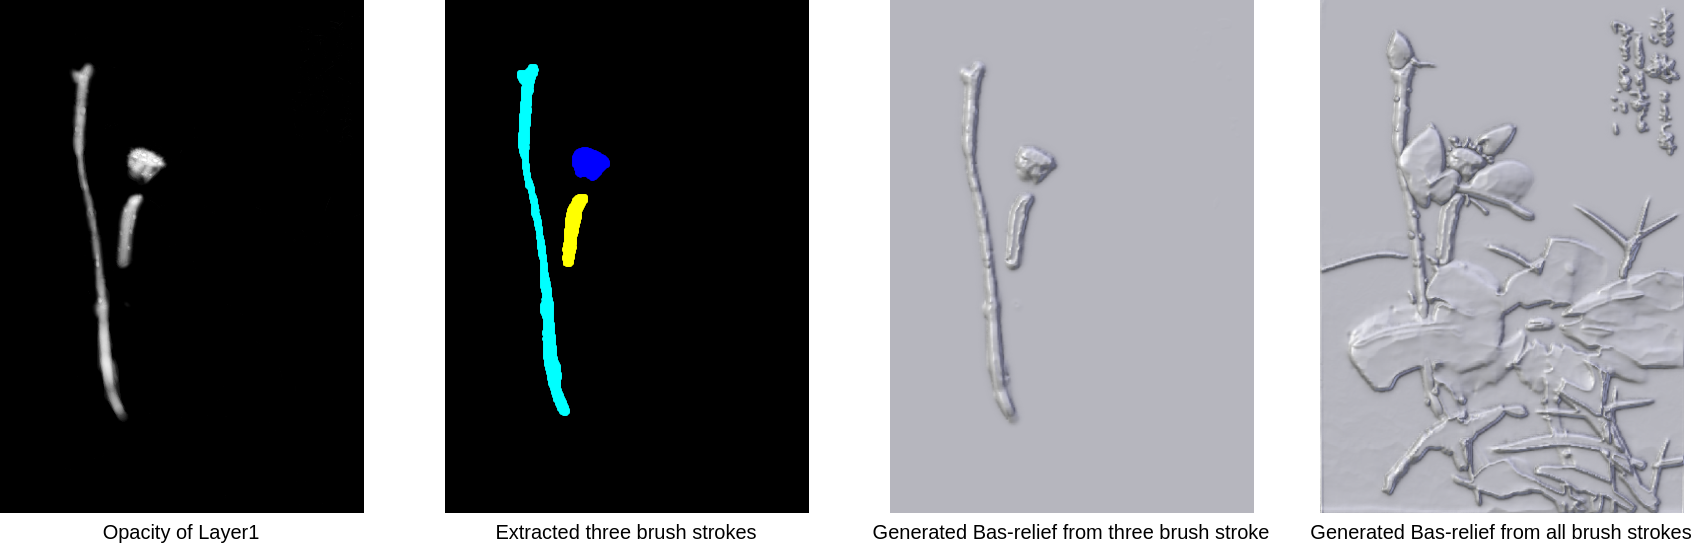
\includegraphics[width=15cm]{strokerelief.png}
	\caption{Bas-relief generation from brush strokes}
	\label{strokerelief}
\end{figure}



\section{Comparison}
This section compares our algorithm against the two most notable 2D image based bas-relief methods, 

The image-based bas-relief approaches\cite{zeng2014region} \cite{kolomenkin2011reconstruction} perform shape from shading algorithm separately on the segmented regions of an image.Most of segmentation methods work on image intensity. Due to lack of information of the spatial relationship, they always suffer from the issues of over-segmentation or incorrect segmentation. As a result, post-processing with user assistance to manipulate the depth maps is necessary. To illustrate this issue, we applied the  orthogonal SFS method \cite{prados2004unifying} on the segmented Rosemaling painting shown in Figure \ref{ETF} to generate the depth maps. It can be seen that there are lots of over-segmentation, or even incorrect segmentation as shown in Figure \ref{overseg}.


\section{Manipulate Bas-relief of stroke}

Moreover, it is desirable to allow the users to manipulate the brush stroke models for secondary creation purposes. We present three approaches based on the generated bar-relief models here.

\textbf{Rising a Stroke}  

For a set of stroke models, we may quantify their depth maps within a specified height scope. The order of strokes may be given by users. Suppose there are n overlapped strokes in a painting, which are sorted in a descending order from 1 to n. Let $S_i$ be the i-th stroke and $h_i(x)$ for the depth of point $x$ within $S_i$ . The depth map of $S_i$ is quantified within the scope of $[0,\rho]$ as,
\begin{equation}
h_i(x)= \frac{(\rho-(i-1)d)h_i(x)}{H_i}
\label{eq:raising}
\end{equation}

where $H_i=\frac{1}{\lvert S_i \rvert}\sum_{x\in S_i} h_i(x)  $, and d controls the depth difference between the successive order of stroke models. To manipulate stroke models, such as raising a stroke, this can be fulfilled by simply changing the order of  as shown in Figure \ref{raising}.
However, the scheme of Eq \ref{eq:raising} cannot settle the issue of two strokes obstructing each other. For example, stroke A partially obstructs the other stroke B while it may be partially obstructed by B. This can be resolved by the following stitching approach.\newline
\begin{figure}[H]
	\centering
	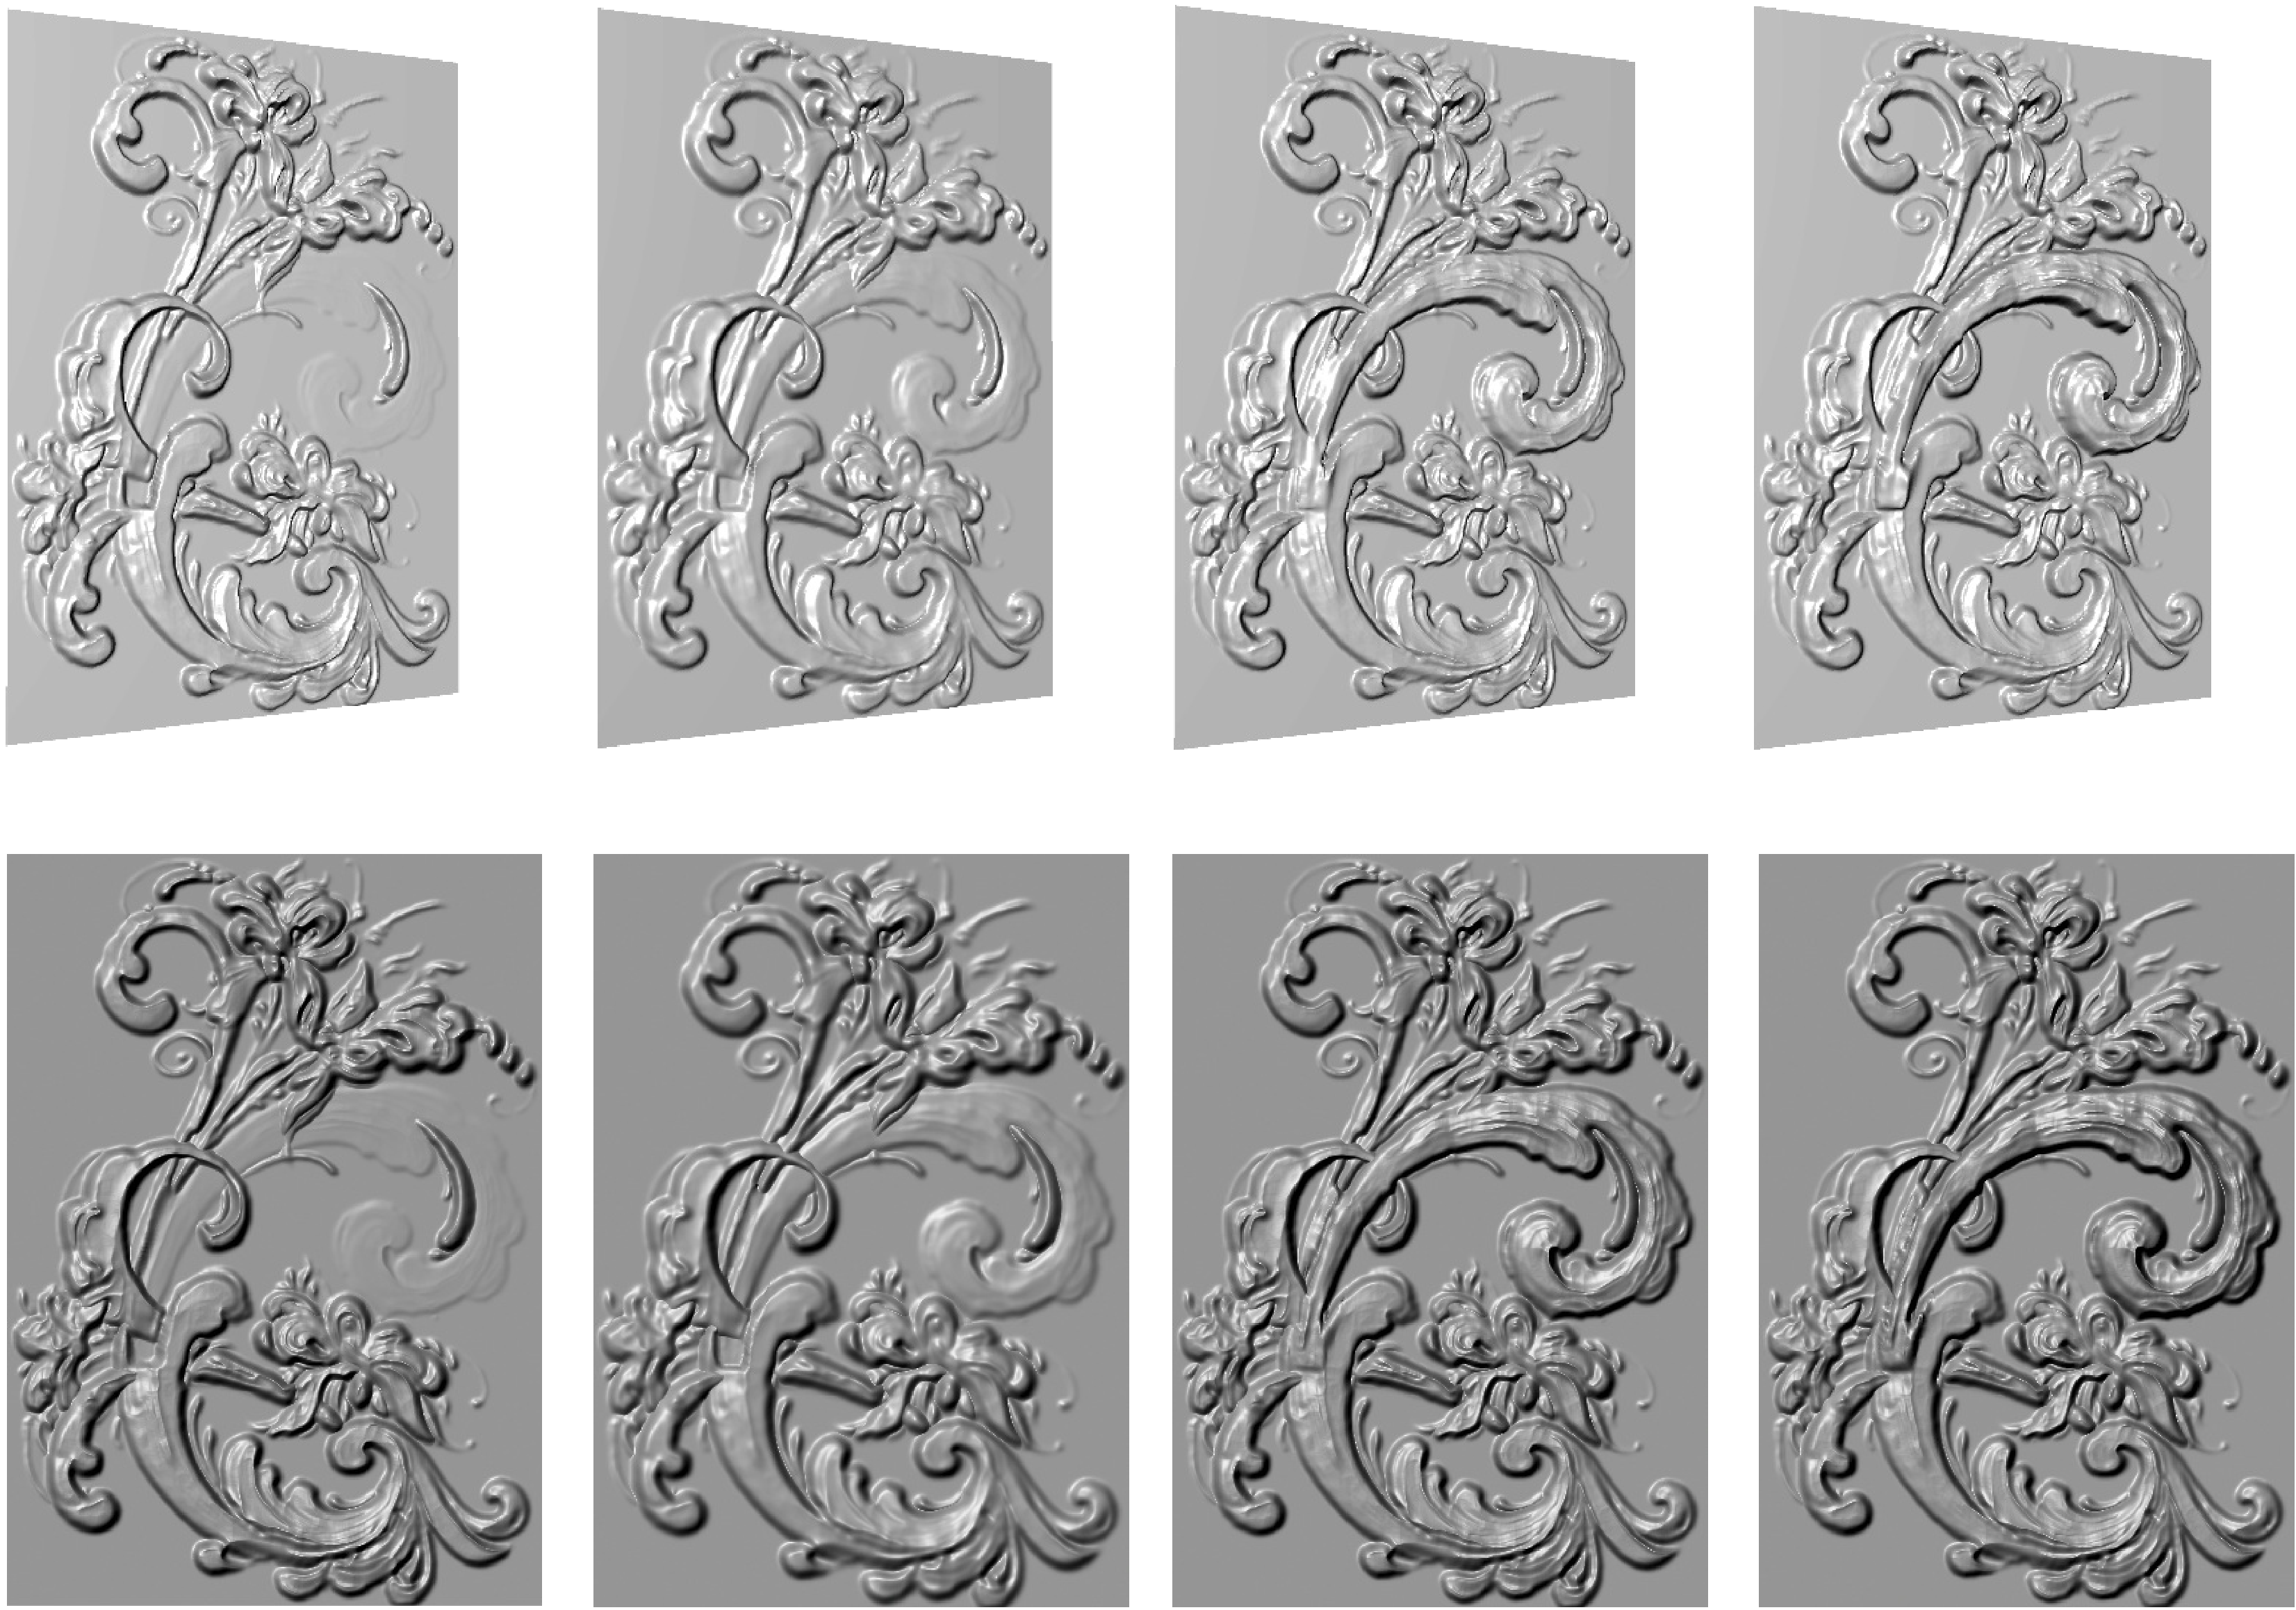
\includegraphics[width=15cm]{risestroke.png}
	\caption{Rising strokes}
	\label{raising}
	\medskip
	The selected strokes is rising from bottom to top in layer order. \\There are 4 layers.
\end{figure}

\textbf{Stitching one Stroke on Another one} 
\newline

For two overlapping strokes $S_i,S_j$, it is desired to stitch the model of $S_i$ on that of the other $S_j$ instead of overlapping their depth maps. This may be accomplished by solving for depth functions $h_i:S_i\rightarrow R $ such that the resulting $h_i$ satisfies stitching positional constraints. We define the set of $ D_{ij} \subseteq \partial S_i \cap \partial S_i $ as the stitching constraints. The depth functions are solved by minimizing the Dirichlet energy, 
\begin{equation}
 \int_{S_i} \lVert \bigtriangledown h_i - \vec{v_i} \rVert ^2 dx ,~ s.t. ~h_i(x)=h_j(x),\forall x \in D_{ij}
 \label{eq:stitch}
\end{equation}

where $\vec{v_i} $ denotes the differential coordinates of the model of $S_i$. Intuitively, this is to update $ h_i(x)$ which keeps close to the depth map of $S_i$ as much as possible while satisfying the positional constraints in a least squares sense. We perform the scheme of Eq \ref{eq:stitch} on the overlapping area of multiple strokes and illustrate all the possible spatial occlusion cases in Figure \ref{stitch}. It can be noted that there are four overlapped strokes to be depicted by using transparency in the Rosemaling painting. In fact there are at most eight occlusion cases as shown in Figure \ref{stitch}. We can further change the shape of these 3D strokes if needed.\newline

\begin{figure}[H]
	\centering
	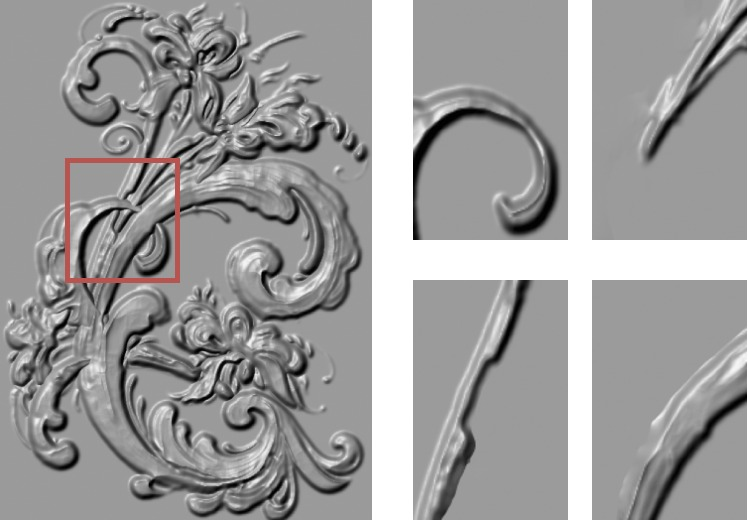
\includegraphics[width=14cm]{edit.jpg}
	\caption{Strokes segmented in selected region}
	\label{shape_edit}
\end{figure}

\begin{figure}[H]
	\centering
	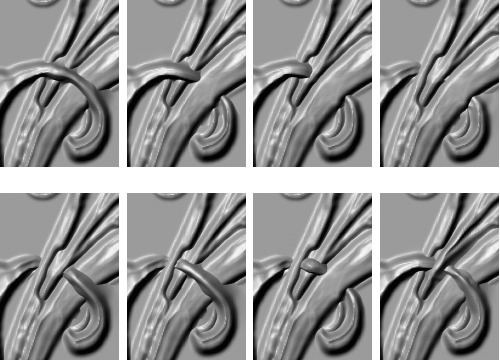
\includegraphics[width=14cm]{stitch.jpg}
	\caption{ The result of stitching strokes}
	\label{stitch}
	\medskip
 The result of stitching one stroke on another one. \\8 cases are highlighted by combining 4 selected strokes 
\end{figure}

\textbf{Changing the Shape of Strokes} 
\newline 

The key point is to determine the changed boundary of strokes on the background plane at first. For a given stroke $S_i$, the boundary of $S_i$ on the plane corresponds to the positional constraints in Eq \ref{eq:stitch}. When users change the boundary $\partial S_i $, the shape of the model of $S_i$ will be changed accordingly based on Eq \ref{eq:stitch}. Painters are used to sketching a skeleton $D_i^{'}$ on the background plane. It requires us to change the boundary of $S_i$ on the plane according to $D_i^{'}$.

To this end, $S_i$ is triangularized by a regular grid on the plane, and its skeleton may be extracted by the Hilditch thinning method \cite{cornea2007curve}. This skeleton can be matched to  $D_i^{'}$ by the lengths. The shape of boundary is deformed on the plane in terms of  $D_i^{'}$ . For an As-Rigid-As-Possible shape deformation \cite{weng20062d} on a plane, we employ the curve Laplacian coordinates on the boundary of $S_i$, $\lVert LV-\delta(V) \rVert ^2 $, where $V$ denotes the vertices of boundary $ \partial S_i $; the mean value coordinates $ \lVert MV \rVert^2 $, where $V$ denotes the vertices within $S_i$; and the positional constraints $D_i^{'}$, $\lVert CV-V^{'} \rVert ^2 $, where $V^{'} \in D_i^{'} $ while $V$ for the updated vertices. The boundary of $S_i$ is updated on the plane by minimizing the following sum of these three terms,

\begin{equation}
\lVert LV-\delta(V) \rVert ^2 + \lVert MV \rVert^2 + \lVert CV-V^{'} \rVert ^2 
\label{eq:shape_edit}
\end{equation}
 
Herein, we expand the matrices of $L,M,C$ through adding zero elements, such that V contains all the vertices of $S_i$ in Eq \ref{eq:shape_edit}. The resulting boundary of $S_i$ is then utilized in Eq \ref{eq:stitch} to update the depth functions of $S_i$ . Figure \ref{shape_edit} shows how to change the shape of the model of $S_i$. \newline 

\begin{figure}[H]
	\centering
	\begin{subfigure}[b]{0.3\textwidth}
		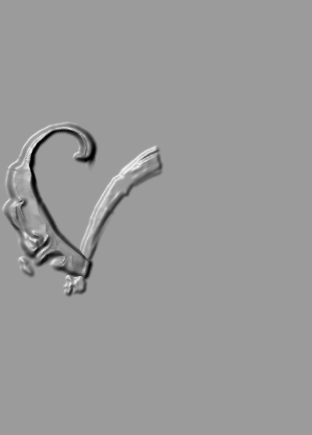
\includegraphics[width=\textwidth]{change.png}
		\caption{selected stroke}
		
	\end{subfigure}
	~  
	\begin{subfigure}[b]{0.3\textwidth}
		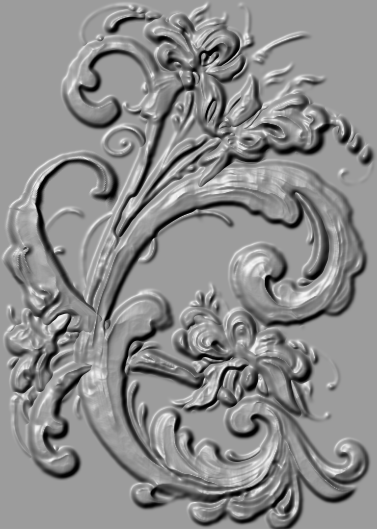
\includegraphics[width=\textwidth]{change1.png}
		\caption{modified depth map}
		
	\end{subfigure}
	\caption{The shape of a stroke is changed}
	\label{shape_edit}
\end{figure}

\textbf{Remark} Compared with image-based bas-relief generation, the main advantage of our approach is the introduction of “3D strokes”. Spatial occlusion offers an important cue in conveying the spatial relationship of the depicted objects and the depth information. Unlike the usual image segmentation problems, our method takes into account spatial occlusion in our stroke segmentation. As a result, over-segmentation and incorrect segmentation are largely eliminated. Moreover, the extracted “3D strokes” both help us sort out the stroke order and provide us a chance to rearrange the strokes as needed. This is in favor of further artistic creation in bas-relief design.


\newpage  \chapter{RESULTS}

\textbf{Implementation}  We modified the published codes of the layer decomposition and MSERs, which are available on GitHub (https://github.com/ CraGL/Decompose-Single-Image-Into-Layers; https://github.com/idiap/mser) ,the differences between our algorithm and the available codes have been explained in Section 4.2.1 and 5.2. Our algorithms were written in Python and vectorized using NumPy/SciPy. Our implementation is not multi-threaded.In our implementation, the parameters in Layer decomposition, ETF field, and MSERs are set the default values as in the original codes.\\ 
\textbf{Performance}  We performed the bas-relief generation on a variety Chinese paintings, and some Rosemaling paintings. We also performed our brush strokes extraction algorithm on some van Gogh's paintings, as described in Section \ref{comparevan}. All the paintings are from the internet.  All the tests were performed on a 6-core of 3.33 GHz Intel Core Xeon CPU with memory of 32 GB(RAM).\\
Table 3 further shows the running time of the proposed approach. Compared to the performance in \cite{tan2016decomposing} and \cite{nister2008linear}, there is no distinct difference. Additionally, the shape from shading algorithm does not consume much time since it depends on the segmented stroke regions. Our implementation is not multithreaded. \\
\textbf{Comparisons}  
As illustrated in section \ref{overview}, our method can be separated into three steps:layer decomposition, brush stroke extraction, bas-relief generation. We compared our work in each step with other alternative methods.\\
For layer decomposition, we compared the our algorithm with the Tan et al's work \cite{tan2016decomposing} in section \ref{comparelayer}, and we demonstrate our modified algorithm can better preserve the smoothness and completeness of brushstorkes in layers. \\
For stroke extraction, we compared our work with Li et al.'s work \cite{li2012rhythmic} in section \ref{comparevan}, and demonstrate that our method have a better performance in brush stroke extraction.\\
For bas-relief generation,we compared our work with Zeng et al.'s work \cite{zeng2014region} in section \ref{compare}, and we demonstrate our algorithm has better performance based on three factors mentioned in Section \ref{2dimagebased} : depth information, silhouettes and edges,fine details. \\
\textbf{Limitations}. We discuss the limitations of this work as related to different steps in the method:
1) Layer decomposition: The paint colors based on building and simplify the  convex hull of input image in RGB space, sometimes, a paint color can be inside of the convex hull which can not be selected. With wrongly picked paint colors, the layer decomposition may not preserve or separate the brush strokes . 
2) Brush stroke: some images can be too complex for proper segmentation, e.g., brush strokes highly blended with  multiple painting colors  (see Figs. 18b and 18c); hence, we cannot form meaningful regions and compute layering.

\begin{figure}[H]
	\centering
	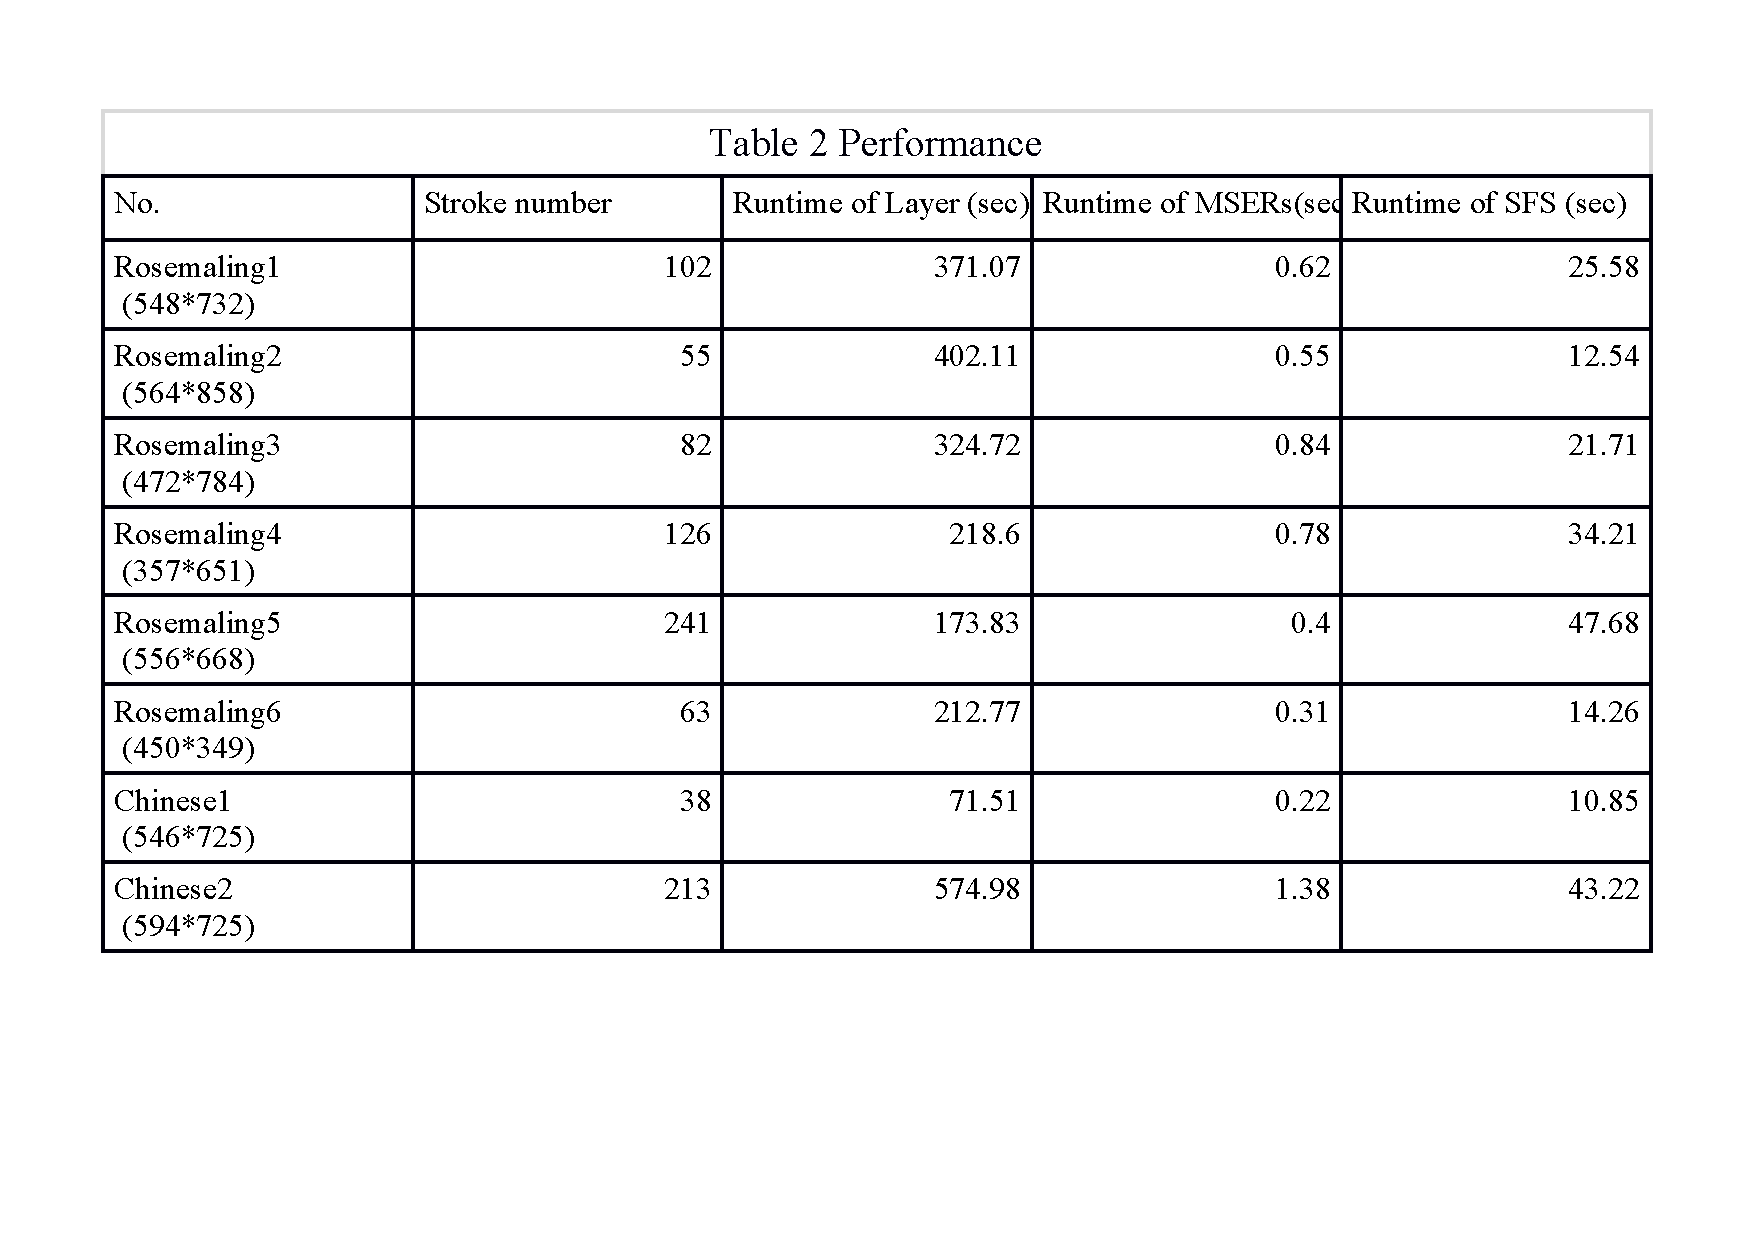
\includegraphics[width=14cm]{performance.pdf}

\end{figure}



\newpage  \section{More Results}
\textbf{More bas-relief generation based on different brush paintings}
\begin{figure}
	\centering
	\includegraphics[page=2,width=17cm]{sup.pdf}
\end{figure}

\begin{figure}
	\centering
	\includegraphics[page=3,width=17cm]{sup.pdf}
\end{figure}

\newpage  \chapter{Conclusions and Future Work}
\section{Conclusions}
Bas-relief is an art form part way between 3D sculpture and 2D painting. We present a new approach for generating a bas-relief from a single Chinese brush painting automatically. \\
Based on layer decomposition , our approach can effectively extract brush strokes from 2D paintings and generate the individual depth maps for bas-relief. We show the superiority of our results by comparing it with alternative works in each step.\\ \\
In summary,our contributions include:
\newline
(1) Extraction of brush strokes. We develop a novel method to extract brush strokes based on paint colors analysis and layer decomposition.  Comparing with previous method brush stroke extraction methods, our method is capable of extracting overlapped brush strokes automatically without the prior knowledge of brush strokes and has higher accuracy. 
\newline
(2) Bas-relief generation of each brush stroke. We develop a novel method which may entirely generated every stroke to a correspond bas-relief surface(a depth map). By doing so, we preserve the feature of the input painting well.\\
(3) Bas-relief generation from opacity. In contrast with previous 2D image based methods, our method use opacity instead of intensity to generate bas-relief, which can better preserve the feature of input painting.\\ 
(4)Our brush stroke extraction technique has other potential uses. We demonstrate the utility of the decomposed brush strokes for image editing. See section \ref{editing}.\\
Our experiments show that our method is able to produce convincing bas-reliefs from a variety of Chinese brush paintings (with human, animal, flower,etc.)  and even some other suitable styles including rosemaling paintings. \\   
\section{Future Work}

Although the proposed algorithm is already capable to generate a bas-relief from a single Chinese brush painting automatically, there is still further work to do, including refinement of our method based on the limitations,and use it in other applications.

\subsection{Refine Current Algorithm}
One future work is to further improve the performance of current algorithm. As we mentioned in section \ref{result}, there are two main limitation: (1) With wrongly picked paint colors, the layer decomposition may not preserve or separate the brush strokes. (2) When brush strokes highly blended with  multiple painting colors, it fails to be extracted faithfully by our current method. \\
We plan to investigate methods to automate the estimation of better color selection from the image contents, e.g., by analyzing the local features. Second, we would study how color composition equation would influence our brush stroke extraction, and refine our method based on it.  

\subsection{Application  }
\textbf{3D painting system}\newline
The concept of 3D painting system was introduced for more than two decades ago.  Hanrahan \cite{hanrahan1990direct} firstly present a 3D painting system that capable of painting on 3D models, but their work didn’t put transparency and fine detailed painting in consideration. \\
From works of  Daily et al. \cite{daily19953d}, 3D painting applied texture map for painting details effect. However, distortion or seams would happen due to 2D parametrization. Meier [1996] first proposed generating brush strokes attached to 3D objects.  Deep Canvas \cite{katanics2003deep}, firstly projected painted strokes on the object’s surface and dynamic 3D camera can be applied which is hard to achieve using traditional 2D paintings. The WYSIWYG NPR system \cite{kalnins2002wysiwyg} focused on algorithmic rendering techniques, which enable artist to achieve silhouette stylization and control hatching directly via a painting interface. Maya Paint Effects (Paint Effects 2011) also projects painted strokes onto the surface of scene geometry and uses them as seed points to create new geometric primitives such as grass or flowers.

\begin{figure}[H]
	\centering
	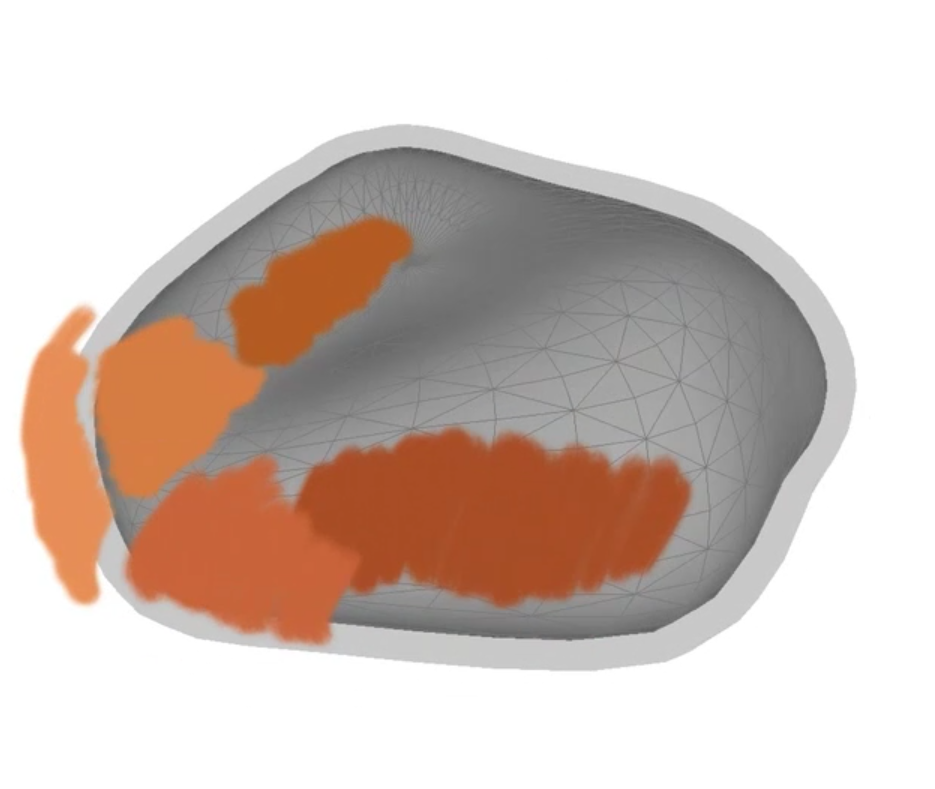
\includegraphics[width=10cm]{level_set.png}
	\caption{3D brush painting on surface level set}
	\label{level set}
\end{figure}

More recently, Overcoat \cite{schmid2011overcoat} introduced an implicit canvas for 3D painting, which enable creating approximate 3D proxy geometry to shape the implicit canvas, it allows us to implement tools for painting along level set surfaces or across different level sets. which means we can project parametric strokes onto the underlying 3D models as showed in Figure \ref{level set}.
These painting systems are focusing on how to paint on surface of known models. In CanvoX \cite{kim2017canvox} extended painting surface to volumetric painting, with GPU-based Octree \cite{lefebvre2005octree}.

With the rapid development of VR systems, it is natural to enable artists to paint in 3D space. In CavePainting \cite{keefe2001cavepainting} firstly create 3D analogy of 2D brush strokes, to create 3D works in a Cave environment. Softwares like Tilt Brush (1) and Quill (2) have recently surged and are now widely accepted by artists to be positioned as a new art form kim's work \cite{kim2017canvox}. For these painting system, quad strips are rendered as painting strokes, which are fully based on user input. \\
\textbf{Application in 3D Painting}\\
With the increasing popularity and development of virtual reality, digital painting on 2D canvases is now being extended to 3D spaces. 3D painting as a new art form are now widely accepted among artists. Software on VR platform make 3D painting more and more intuitive for 2D painters.   
We aim to build a system which enable artist to transfer a given 2D Chinese painting to 3D painting, in a way that gives creative freedom to the artist while maintaining an acceptable level of controllability based on the given 2D Chinese painting.\\
We address this problem into four main steps: \\
First, segment strokes from the given 2D Chinese painting. Since in 3D painting, strokes are placed in 3D space based on user input, to mimic such effect, successful strokes segmentation is quite essential. Brush strokes may have high diversity of colour, so layer decomposition may need to be applied. \\
Second, stroke refinement, since brush strokes may be over segmented or under segmented, stroke need to be refined. A refinement method based on user input need to be applied. \\
Third, transfer 2D strokes to 3D strokes, simulate the effect the 3D stroke with supplied 2D stroke, and 3D volumetric painting would be applied \cite{kim2017canvox}. \\
Fourth, 3D strokes placement, based on the layer order and user inputs, we place and blend 3D strokes in 3D space. \\
\section{Proposed timescale for the work:}
Refine the first step of layer decomposition, with the coherent edge of the given 2D brush painting, iteratively calculate the paint colors. (6 weeks)\\
Stroke segmentation into a hierarchical structure, currently,  hierarchical clustering are in consideration. (4 weeks)\\
Design the user interface for refine the stroke segmentation. (4 weeks)\\
With given segmented strokes, generate corresponding mesh, with detail and style preserved. (4 weeks)\\
Design the interface for user input, in which high relief can be placed naturally in 3D space while maintaining an acceptable level of controllability. (4 weeks)\\
Optimization.  (4 weeks)
\newline

\begin{table}[H]
	\centering
	\caption{ Schedule of Future Research Plan}
	\label{my-label}
	\begin{tabular}{|l|l|}
		\hline
		\textbf{Research Activity} & \textbf{Target Completion Date} \\ \hline
		\begin{tabular}[c]{@{}l@{}}Refine current algorithm \end{tabular} & 11/12/2017 \\ \hline
		\begin{tabular}[c]{@{}l@{}}Design the user interface for refine the\\ stroke segmentation.\end{tabular} & 01/3/2018 \\ \hline
		\begin{tabular}[c]{@{}l@{}}3D stroke analogy design and 3D stroke\\ placement design .\end{tabular} & 01/04/2018 \\ \hline
		Optimization. & 01/05/2018 \\ \hline
		Write final Thesis for PhD graduation & 01/10/2018 \\ \hline
	\end{tabular}
\end{table}
%\newpage  \chapter{Future Work}
In the future, At first,we will study a wider range of paintings and investigate the issues of layer decomposition and stroke segmentation. Different paintings have different stroke patterns. Understanding the rules will improve the success rate of a wider range of paintings. Proper automatic color separation in the overlap regions is not trivial which will also be studied in the future.Second we would try to build high relief based on current algorithm, and based on the depth of high relief , we would try to generate 3D brush painting effects from 2D brush painting, as showed in Figure \ref{Autumn Tree}.
\begin{figure}[H]
	\centering
	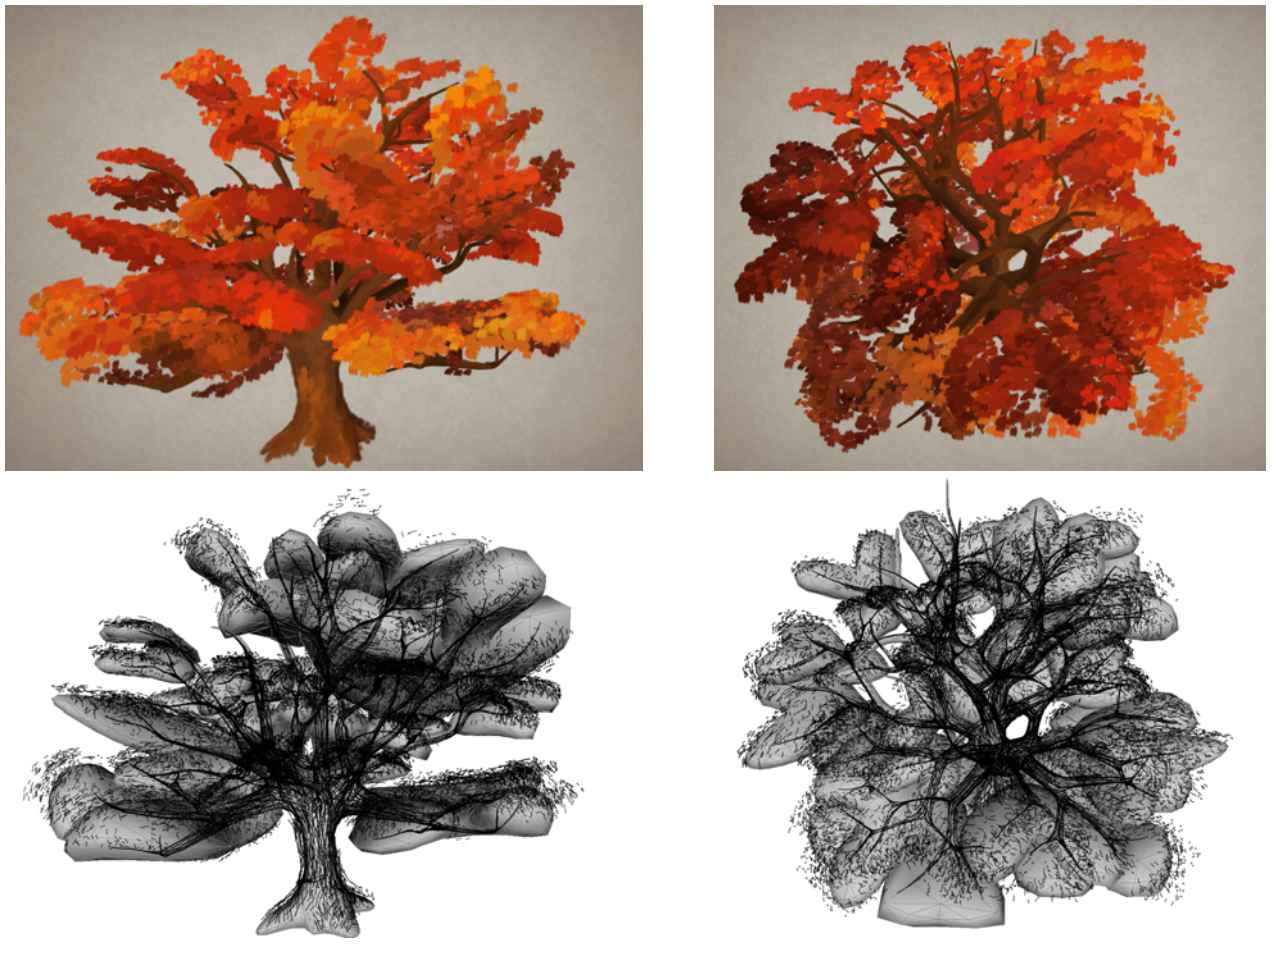
\includegraphics[width=12cm]{autumn_tree.png}
	\caption{3D brush painting : Autumn Tree}
	\label{Autumn Tree}
	\medskip
	The top row shows two different views of a painted tree. The bottom row shows the respective proxy geometry with paint stroke paths on top.
\end{figure}
\section{From 2D Brush Painting to 3D Brush Painting}
\subsection{Abstract} 
With the increasing popularity and development of virtual reality, digital painting on 2D canvases is now being extended to 3D spaces. 3D painting as a new art form are now widely accepted among artists. Software on VR platform such as Tilt Brush and Oculus Quill make 3D painting more and more intuitive for 2D painters.   
We aim to build a system which enable artist to transfer a given 2D brush painting to 3D painting, in a way that gives creative freedom to the artist while maintaining an acceptable level of controllability based on the given 2D brush painting. 

We address this problem into four main steps: 
first, segment strokes from the given 2D brush painting. Since in 3D brush painting, strokes are placed in 3D space based on user input, to mimic such effect, successful strokes segmentation is quite essential. Brush strokes may have high diversity of colour, so layer decomposition may need to be applied. 
Second, stroke refinement, since brush strokes may be over segmented or under segmented, stroke need to be refined. A refinement method based on user input need to be applied. 
Third, transfer 2D strokes to 3D strokes, simulate the effect the 3D stroke with supplied 2D stroke, and 3D volumetric painting would be applied \cite{kim2017canvox}. 
Fourth, 3D strokes placement, based on the layer order and user inputs, we place and blend 3D strokes in 3D space. 

\subsection{Aims and Objectives}
With given 2D brush painting, we aim to design a new approach to generate a 3D brush painting. With such a goal, we need to achieve following:
1. Based on edge and region segmentation, retrieve the reasonable palette colours from input 2D brush painting. 
2. Efficient hierarchical segmentation for brush strokes based on layer decomposition. 
Simulate different scale of brush strokes based on hierarchical segmentation and dynamic branch cutting.
3. Refine stroke segmentation based on user input.
4. Generate correspond 3D brush strokes from 2D brush strokes. 
5. Place and deform 3D brush strokes based on user input.
6. The 3D brush painting must preserve the style and placement order of original 2D brush. 
\subsection{Background and Literature Review:}  

\textbf{ Stroke based rendering:} \newline

The difference between primary space (the 3D world in which objects live) and secondary space (the 2D canvas on which depictions of those objects are created) was highlighted by \cite{schmid2011overcoat}. 

The field of non-photorealistic rendering (NPR) has developed many stylization on 2D canvas. Although traditional photorealistic rendering research focuses on the primary space (e.g., scene representation, visibility determination, global illumination), the NPR community first approached the problem from the opposite direction by focusing entirely on the secondary space of the 2D canvas \cite{hanrahan1990direct}. 

Haeberli’s interactive “Paint By Numbers” system \cite{haeberli1990paint} started the research of stroke based rendering, which proposed a method to fills a 2D canvas with brush strokes when parametric brush stroke are controlled based on given photograph. And similar works which provide automatic approach by placing discrete elements such as paint strokes or stipples to create nonphotorealistic imagery are described stroke-based rendering \cite{hertzmann2003survey} . Interactive stylization of images, video, and animations \cite{lu2010interactive} has also been done.  
These researches mainly focus on how to implement different expressive styles on canvas which algorithmic mapped from primary space. \newline

\textbf{3D painting system:}\newline

The concept of 3D painting system was introduced for more than two decades ago.  Hanrahan \cite{hanrahan1990direct} firstly present a 3D painting system that capable of painting on 3D models, but their work didn’t put transparency and fine detailed painting in consideration. 

From works of  Daily et al. \cite{daily19953d}, 3D painting applied texture map for painting details effect. However, distortion or seams would happen due to 2D parametrization. Meier [1996] first proposed generating brush strokes attached to 3D objects.  Deep Canvas \cite{katanics2003deep}, firstly projected painted strokes on the object’s surface and dynamic 3D camera can be applied which is hard to achieve using traditional 2D paintings. The WYSIWYG NPR system \cite{kalnins2002wysiwyg} focused on algorithmic rendering techniques, which enable artist to achieve silhouette stylization and control hatching directly via a painting interface. Maya Paint Effects (Paint Effects 2011) also projects painted strokes onto the surface of scene geometry and uses them as seed points to create new geometric primitives such as grass or flowers.

\begin{figure}[H]
	\centering
	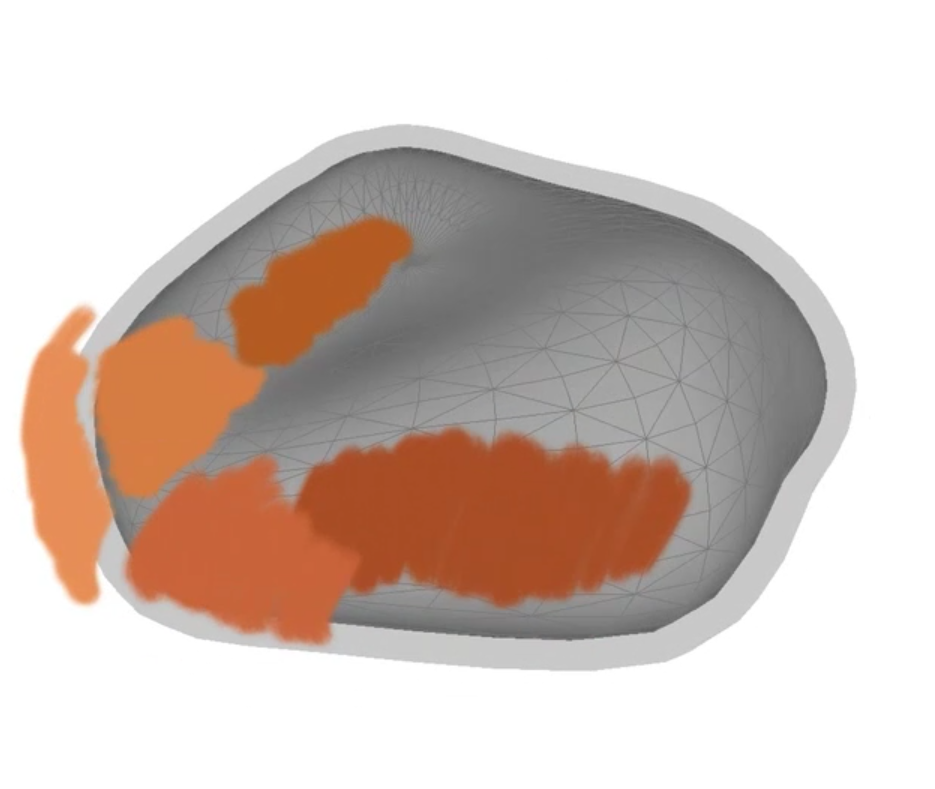
\includegraphics[width=10cm]{level_set.png}
	\caption{3D brush painting on surface level set}
	\label{level set}
\end{figure}

More recently, Overcoat \cite{schmid2011overcoat} introduced an implicit canvas for 3D painting, which enable creating approximate 3D proxy geometry to shape the implicit canvas, it allows us to implement tools for painting along level set surfaces or across different level sets. which means we can project parametric strokes onto the underlying 3D models as showed in Figure \ref{level set}.
These painting systems are focusing on how to paint on surface of known models. In CanvoX \cite{kim2017canvox} extended painting surface to volumetric painting, with GPU-based Octree \cite{lefebvre2005octree}.

With the rapid development of VR systems, it is natural to enable artists to paint in 3D space. In CavePainting \cite{keefe2001cavepainting} firstly create 3D analogy of 2D brush strokes, to create 3D works in a Cave environment. Softwares like Tilt Brush (1) and Quill (2) have recently surged and are now widely accepted by artists to be positioned as a new art form kim's work \cite{kim2017canvox}. For these painting system, quad strips are rendered as painting strokes, which are fully based on user input. 

It is natural to think how to transfer 2D brush paintings to 3D brush painting while preserving its original style. \newline

\textbf{Outline of Proposed Methodology: }\newline

Layer decomposition:  Digital painting with different layers is an integral feature of digital image editing software, such as Photoshop and Sketchbook. Layers offer an intuitive way to edit the colour and geometry of components and localize changes to the desired portion of the final image. Without layers, brush stroke segmentation becomes extremely challenging, since they can overlap and blend with each other. So, at first, we decompose the given 2D brush painting into several layers, which layer contains same colour while each pixel has different transparency. 

Stroke segmentation: As mentioned above, to transfer 2D strokes to 3D strokes, we need to segment each stroke on the painting, inspired by the level set representation of 3D painting in Overcoat, we would segment brush strokes into a hierarchical structure.  

Stroke refinement: To maintain the style of 2D brush painting, successful stroke segmentation is essential for the next step. Wrong segmentation would happen in the process of automatic segmentation, to refine the strokes, user input would be applied. Since the strokes would be a hierarchical structure, hierarchical cut might be applied as well. 

3D stroke analogy: Given segmented strokes, we would create correspond 3D strokes, in which 3D volumetric painting would be applied \cite{kim2017canvox}.

Stroke placement: After generation of 3D stroke analogy for each 2D stroke, a user interface would be supplied for stroke placement.  \newline

\textbf{Proposed timescale for the work:}\newline

Refine the first step of layer decomposition, with the coherent edge of the given 2D brush painting, calculate the palette colour. (4 weeks)

Stroke segmentation into a hierarchical structure, currently, SLIC and hierarchical clustering are in consideration. (4 weeks)

Design the user interface for refine the stroke segmentation. (4 weeks)

3D stroke analogy design. With given segmented strokes, generate corresponding 3D stroke, with detail and style preserved. (6 weeks)

3D stroke placement design. Design the interface for user input, in which 3D strokes can be placed naturally in 3D space while maintaining an acceptable level of controllability. (3 weeks)

Optimization.  (4 weeks)
\newline

\begin{table}[H]
	\centering
	\caption{ Schedule of Future Research Plan}
	\label{my-label}
\begin{tabular}{|l|l|}
	\hline
	\textbf{Research Activity} & \textbf{Target Completion Date} \\ \hline
	\begin{tabular}[c]{@{}l@{}}Design and implement the proposed \\ refinement work. Do experiments accordingly.\end{tabular} & 01/08/2016 \\ \hline
	\begin{tabular}[c]{@{}l@{}}Design the user interface for refine the\\ stroke segmentation.\end{tabular} & 01/09/2016 \\ \hline
	\begin{tabular}[c]{@{}l@{}}3D stroke analogy design and 3D stroke\\ placement design .\end{tabular} & 01/12/2016 \\ \hline
	Optimization. & 01/01/2017 \\ \hline
	Write final Thesis for PhD graduation & 01/06/2018 \\ \hline
\end{tabular}
\end{table}
\newpage  \bibliographystyle{unsrt}
\bibliography{ref}

\end{document}